\documentclass[pageno]{jpaper}

%replace XXX with the submission number you are given from the ISCA submission site.
\newcommand{\IWreport}{2015}
\newcommand{\project}{IMAPSec }
\newcommand{\projectnospace}{IMAPSec}

\usepackage[normalem]{ulem}
\usepackage{listings}
\lstset{language=Python}
\usepackage{multirow}

\begin{document}


\title{Making (Secure) FETCH Happen:
\\ \vspace{2 mm} {\large End-to-End Metadata Security for IMAP}}

%  Providing End-to-End Metadata Security for IMAP
% \title{\project: Secure, Backwards-Compatible Storage for Metadata-Secure Messaging Systems
% \\ \vspace{2 mm} {\large Invisibly Protecting Content and Metadata On Johnny's Behalf}}

\author{Erica Portnoy}

\date{}


\begin{titlepage}
\begin{center}

{ \huge \bfseries Making (Secure) FETCH Happen \\[0.5cm] }

{\LARGE End-to-End Metadata Security for IMAP}\\[1.5cm]

{\large Erica Portnoy\\
2015\\
Advised by Prof. Edward Felten and Dr. Joseph Bonneau\\
Submitted to: Princeton University\\
Department of Computer Science}\\[1.5cm]

{\large This Thesis represents my own work in accordance with University Regulations.}\\[6cm]

{\large Date of Submission: April 30, 2015}


\end{center}
\end{titlepage}


\thispagestyle{empty}

\vspace*{2 cm}

\begin{abstract}
Although communication metadata is known to be intrusive, most end-to-end encryption solutions focus only on hiding the contents of messages. Yet who a user is talking to and when is information as sensitive as the contents of the message. While end-to-end metadata security solutions exist for message transport, existing solutions lack the multi-device synchronization that IMAP provides. Without providing full feature parity with legacy email technologies, a metadata-secure protocol cannot hope to achieve ubiquity. To that end, we present \projectnospace, a client-side extension of the IMAP protocol held to rigorous standards of feature parity without sacrificing on security. With \projectnospace, existing IMAP clients can be invisibly upgraded to provide metadata security for email storage and synchronization, enabling the rollout of end-to-end metadata secure messaging.
\end{abstract}

\newpage

\tableofcontents

\newpage

\section{Introduction}

Today, most email is hosted by cloud providers. Unfortunately for users, this means that information about who they're talking to, when they're talking to those people, and what they're saying to each other is readily available to any interested company, government, or advertiser. Given that a modern threat model must account for the mail provider as an adversary, then only an end-to-end (E2E) solution will provide adequate security. Furthermore, even encrypting the contents of the email will protect only a small portion of the full breadth of sensitive information: the metadata of who is communicating and when is equally important to protect. Fortunately, recent projects have emerged to add protections for metadata into the communication security toolkit. Yet these projects lack a key feature to achieve full feature parity with insecure messaging solutions: support for multi-client synchronization and storage across all of a user's devices.

Full feature parity is not merely a luxury. To achieve ubiquitous end-to-end metadata security, we cannot place any burden on users to alter their present actions or expectations of available functionality. Our target user is familiar with modern email and its usage, but cannot be expected to have any security expertise or specialized knowledge. A parallel model in the instant messaging space is present in applications such as iMessage and WhatsApp, both of which provide E2E encryption to their users, but incur no visible differences in functionality or usability. With this project, we enable this manner of full feature parity for a messaging system that is metadata-secure.

\project is a solution that allows users to access their messages across their devices in a way indistinguishable to the user from current IMAP, but without revealing email content or metadata to the IMAP server. Requiring only modifications on the client machine, it maintains the IMAP interface presented to a mail application. Thus, it achieves the following properties:

\begin{itemize}
  \item Backwards compatibility from the perspective of both the client software and the user
  \item Protection of end-to-end metadata security, including from the IMAP server
  \item Support for the synchronization of multiple clients with the server
\end{itemize}

Furthermore, it does so in a way largely consistent with current expectations for time and space requirements. With these features combined, \project enables the silent upgrade of modern email systems to include metadata security.

% Garfinkel et al. \cite{garfinkel} talk about ``How to make secure email easier to use,'' and Ruoti et al. talk about dangers in automatic encryption \cite{ruoti}.

\section{Relevant technologies and related work}

While current technologies do not provide features that satisfy our stated goals, existing protocols and applications form the ecosystem in which \project resides.

\subsection{Classical email}
Modern email is composed of two distinct protocol stages: sending and transport, and storage and retrieval, shown below in a diagram from \cite{smtp_imap}.

\begin{center}
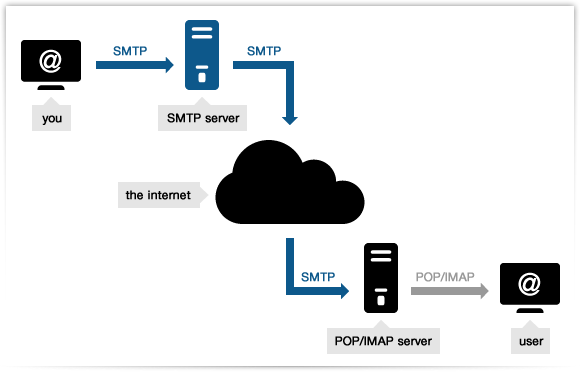
\includegraphics[width=0.6\textwidth]{smtp_imap}
\end{center}

To send an email, the sender's machine sends a request to an SMTP server acting on its behalf, which relays the message through other SMTP servers until it reaches the recipient's destination server. At that point, the recipient's machine retrieves the email from the server using either POP or IMAP.

\subsubsection{Mail Sending and Transport}
The standard sending and transport protocol is Simple Mail Transfer Protocol (SMTP), first defined in RFC 821 \cite{postel1982rfc} in 1982, and most recently updated in RFC 5321 \cite{klensin2008rfc}. SMTP is an application-layer Internet protocol. In SMTP, a user runs a mail client, called a mail user agent (MUA). This MUA submits mail to a mail server (the mail submission agent, MSA) on either port 25, 587, or with SSL enabled on 465. The MSA passes the message to a mail transfer agent (MTA), which is often on the same machine as the MSA. The MTA then looks to transfer the message to the recipient's mail exchanger (MX). It does this by looking up the recipient's domain in the Domain Name System (DNS). The MTA then sends the email over the Internet to the MX. The MX then sends the email to the recipient's mail delivery agent (MDA). The MDA will either store the message or continue to forward it to another MDA. Upon arriving at its final MDA, the SMTP portion of email delivery is complete.


\subsubsection{Mail Retrieval, Storage, and Synchronization}
\label{legacyimap}
Once a message has arrived at an MDA, the recipient's MUA must retrieve the message. For this, most MUAs use either POP or IMAP. Post Office Protocol (POP) is a simple protocol that enables downloads and deletions, and is most often used when a single client is interested in retrieving mail from an MDA \cite{reynolds1984post} \cite{myers1996post}. The Internet Message Access Protocol (IMAP) is a more complex protocol that enables multiple clients to be connected to and modifying the same mailbox, and has come into more widespread use in recent years \cite{rfc3501}.

The current version of IMAP is IMAP 4 revision 1 (IMAP4rev1). An IMAP client connects to an IMAP server over port 143, or over 993 if using SSL. The protocol allows a rich set of commands and actions, enabling clients to create, delete, and rename mailboxes, check for new messages, permanently remove messages, set and clear flags that facilitate multi-client synchronization, and more. Communication is structured in a command-response model, where all messages sent from the server are direct responses to requests from the client. Commands can be tagged with various labels, including OK to indicate success and BAD to indicate a malformed command, or they can be untagged. While not explicitly required by the protocol, a standard client implementation will use the provided commands to locally duplicate the server's state, thereby causing state to be replicated across the server and one or more clients, with all clients synchronized via the server. Many modern languages, including Python, include a library for sending commands to an IMAP server.

\subsection{Non-metadata End-To-End (E2E) Security}
While the standard email protocols are not secure in and of themselves, there have been numerous attempts over the years to provide secure alternatives. Link encryption (sending over SSL/TLS) has been the most widely adopted, but suggestions for messaging with E2E security have been proposed to varying levels of adoption and with a diverse range of feature inclusion \cite{unger2015sok}. These features include synchronicity, deniability, and forward/backward secrecy.


\subsubsection{Pretty Good Privacy (PGP)}
PGP is the classic example of an end-to-end email encryption tool, and also the classic example of a usability failure. Defined in RFC 4880 as the OpenPGP standard, it provides users the ability to sign, encrypt, and decrypt data using a combination of symmetric and public key cryptography \cite{callas2007openpgp}. Unfortunately, usability studies continue to find that users of the system are unable to use it properly, with errors ranging from key management issues to the inability to encrypt a message \cite{whitten1999johnny} \cite{sheng2006johnny}. Even for users for whom communication secrecy is vital to operational success, such as people working on sensitive projects at a non-violent, direct action organization, it is still easy to make errors that compromise the security of the emails \cite{gaw2006secrecy}.

\subsubsection{Yahoo! E2E Extension}
In the past year, major mail providers have begun to express public interest in providing E2E encryption for their users. In particular, Yahoo! recently released the source for a browser extension (based on one developed by Google) that modifies the Yahoo! webmail client to integrate E2E \cite{yahooe2e}. It handles key management automatically, decreasing the cognitive load on the user. Since it is developed in-house, it has both the design resources and engineering manpower of a modern large technology company.

\subsubsection{Messaging Apps}
Some of the most usable and widespread E2E solutions are not for email, but for mobile chat. Apple's iMessage application encrypts messages E2E, although their key management system is unknown and may therefore be invisibly compromised \cite{imessage}. Their messaging system is not only usable: it is a widely-adopted example of a smooth transition to an updated protocol without problematic updates to the user experience. Signal and TextSecure, from Open Whisper Systems, provide a similar experience, but avoid iMessage's public key infrastructure dependency by using instead a modified version of Off-the-Record Messaging (OTR), which can use solutions to the socialist millionaires problem in place of relying on a previously known public key \cite{borisov2004off}. The socialist millionaires problem is a zero-knowledge construction where multiple parties would like to test private values for equality without revealing any information to the other party other than the result of the test. Crucially, Signal and TextSecure enable asynchronous messaging by preemptively generating and sending signed key exchange messages \cite{whisper}. They thereby also provide forward secrecy and deniability in an asynchronous setting. The technology used to implement their solution was implemented in the popular messaging application WhatsApp as well \cite{whatsapp}.


\subsection{E2E Metadata Security for Transport}
While messaging applications have largely saturated the space of ways to ensure content confidentiality and communicants authentication, metadata security requires an additional layer of protection. For example, if we were to see the following inbox contents, we do not need to see the contents of the emails to gain some understanding of the events that transpired.

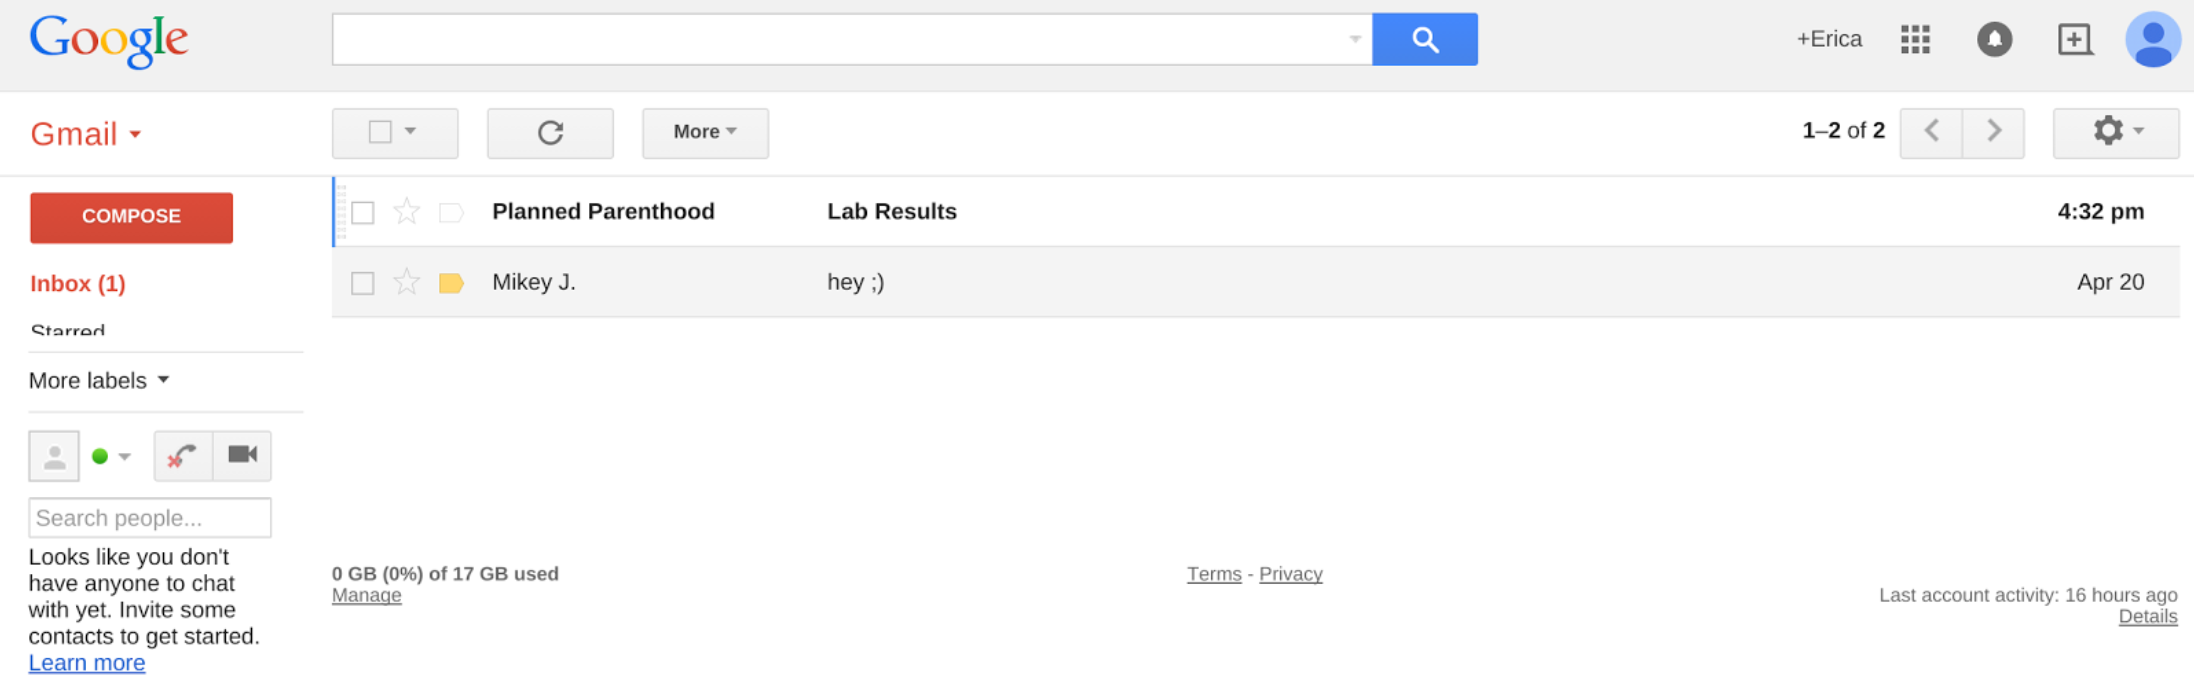
\includegraphics[width=\textwidth]{planned}

Who a person is communicating with and when they do so can reveal as much information, if not more, than the contents of the messages. But it is difficult to secure metadata. Communication protocols generally rely on the inclusion of a FROM header to know the return address, as well as to prevent spam. And the server that delivered a message will certainly know when it was delivered, as well, meaning that an observer with the ability to correlate the timing of messages can recover the identities of the communicants. To achieve metadata-security, a protocol that is oblivious to the sender's identity must include a solution for spam mitigation, such as a proof-of-work algorithm. It must also provide some anonymity in its routing.

These challenges have been addressed more thoroughly in the space of providing transport anonymity, and particularly for Internet routing. Tor, a system for anonymizing Internet traffic, sees about 2.5 million users per day \cite{torusers}. As these figures have taught us, Tor users demonstrate a desire to hide the metadata of their online activities. Anonymous remailers use Tor-like forwarding, but have not seen as wide adoption. Pond, a non-email messaging application, provides forward secure asynchronous messaging that does not leak traffic information ``except [to] a global passive attacker.'' \cite{pond}. There also exist SMTP servers that run as Tor hidden services, essentially bootstrapping their mail anonymity off of Tor's anonymity \cite{onionmail}.


\subsubsection{Mailpile and SMTorP}
While anonymous servers abound, mail clients are generally left to the user's preference. Mailpile, in contrast, is a mail client designed with a goal of integrating security features into the user experience \cite{mailpile}. It integrates key management into its main contact management system, and includes visual indicators (green locks) to denote secure messages in the style of https in browser URL bars. Furthermore, Mailpile contains an experimental plugin (SMTorP) that enables users to opportunistically communicate with other users of the plugin in a metadata-secure manner, by sending messages over Tor \cite{smtorp}. SMTorP is semantically similar to SMTP, except that the receiving client runs an SMTP server on the same machine as the mail client, set up as a Tor hidden service. When used in this fashion, an email is sent to the recipient's .onion address (the address of the hidden service) instead of a human-chosen address. The Mailpile authors note that running an SMTP server on a Tor hidden service might be a security liability, since this opens the client to potentially malicious traffic. Additionally, the alphanumeric string preceding the .onion address is not human-memorable. To address the lack of human-memorability in addresses, the authors consider having users advertise their addresses in the headers of legacy emails that they send, as an invisible upgrade rollout strategy. Clients could then advertise their upgraded status through these headers, invisibly switching to the new protocol when both communicating parties have received the .onion address associated with the legacy email address. The protocol also uses hashcash, a proof-of-work algorithm, to defend against spam (bulk commercial unsolicited email).


Through these tools, the transport mechanism becomes more secure. Yet for all of these, messages are assumed to be transient or remain only on the client device. This is unacceptable behavior to a typical modern user. Modern users expect their emails to be stored on a server and available to them from multiple clients -- from their computers, mobile devices, and on the Web. We could perhaps imagine a situation without an IMAP-like protocol, where the machine that receives messages is also a trusted webmail server and therefore need not perform any synchronization. Although webmail is popular, such a solution is still a feature rollback, and is therefore unacceptable ideologically given our stated aims. To ubiquitize secure email, we must develop a storage and synchronization solution that protects messages at rest without compromising the benefits of secure transport protocols.


\section{Threat model}

Given the modern state of pervasive surveillance, it is appropriate for our threat model to err on the side of paranoia. The IMAP protocol uses a central server to provide mail storage functionality to multiple clients. Popular mail providers such as Gmail, Yahoo! Mail, and Hotmail provide their users not only with servers, but with client functionality as well. \project assumes an untrusted network and an untrusted server, but a trusted client. The attacker controls the server, so we do not expect it to guarantee availability. The attacker may both passively analyze any data it is sent for timing or content information, and reply dishonestly to client requests. The IMAP servers of multiple users may collude. A network adversary, either passive or active, may collude with the adversary running the IMAP server. Either of these may themselves be users of \projectnospace, and attempt to gain information from communicating with a target user. All clients of the same account on a mail server have equivalent access privileges. These adversaries may attempt to determine the contents of a message, the communicants, and when a message was received (in order to determine the other two). We make the prior assumption that messages were initially sent to the client in a metadata-secure manner. A client should be able to identify and reject misinformation sent to it by the server.


\section{Target user}
\label{targetuser}

To achieve ubiquitous adoption, we must not place high technical expectations on our target user. Our target user is non-technical but experienced with modern email tools. Given a standard mail client, the user can easily send and receive emails, and handle advanced email features like folders and labels. They may need to send files as attachments over emails, and do not wish to receive spam. They access their email from a variety of devices, including their desktop, smartphone, and a web browser. The user must notice no difference between their legacy email experience and their metadata-protected email experience.


\section{Design overview}
To meet all aforementioned requirements, we present \projectnospace, a client-only extension to the IMAP protocol that provides metadata privacy-preserving storage for multiple \project clients. In \projectnospace, emails received at the client are fully encrypted (including mail headers), indexed, and uploaded to a specialized mailbox in the IMAP server. This hides sender and recipient information from the IMAP server. Encryption is based on a passphrase and generated salt, using scrypt as a key derivation function. A special-use ``INDEX'' message is stored in the mailbox as well, and tracks metadata for the client such as the apparent mailbox that a message is in (called a pseudo-mailbox, and visible only to clients, not the server). A special-use ``LOCK'' message is used to allow multiple clients access to the same mailbox, in keeping with IMAP's design principles. Message arrival times are hidden from the server using a combination of scheduling, mixing, fake decoy messages, and techniques drawn from oblivious RAM. \project provides rollback detection for both messages and the index, using version numbers saved client-side and message hashes stored server-side. It is robust to client failure in any state.

\section{Email Usage Measurements}
To determine various factors such as how often to update and how large a fake message should be, an implementation of \project should measure and dynamically learn these values for actual incoming messages for each particular user. The usage patterns of the author, an American university student, are as follows.

\subsection{Size}

Email sizes roughly follow a ``long tail'' distribution (where the integral of the graph of distribution of sizes is logarithmic). Sizes below are calculated on a mailbox with a total of over 77,000 messages, and cumulative number of messages below a particular size are graphed.

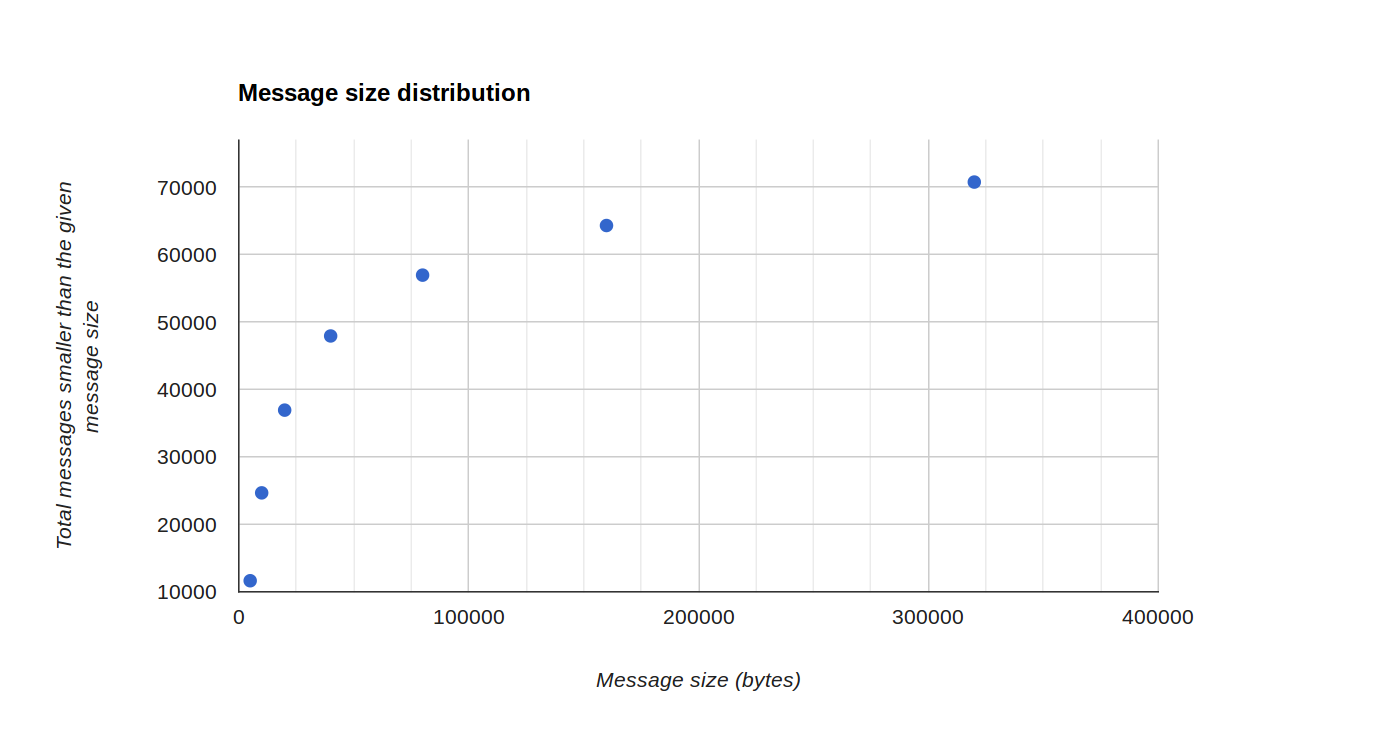
\includegraphics[width=\textwidth]{message-size-dist}

\subsection{Timing}

The following graphic displays message timestamps per day of the week and hour of the day, in a Github-style ``punchcard'' format \cite{punchcard}. In this graphic, day-time combinations that receive more messages are shaded darker, and with larger circles.

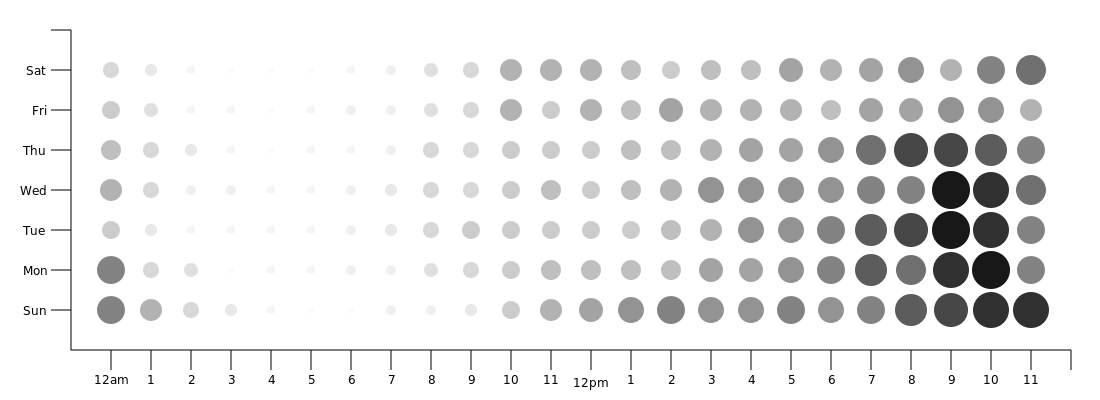
\includegraphics[width=\textwidth]{punchcard}

We can also find message interarrival times \---- that is, the distribution of the length of time between message arrivals and sends. Since this data was taken from the Gmail ``All Mail'' mailbox, it includes both received and sent messages, as the set of all messages synchronized to an IMAP server would. Plotted on a linear scale, the ``long tail'' distribution is once again evident; since it has an extremely high initial slope, we show it also on a logarithmic scale for clarity. The vertical axis shows the total number of messages with inter-message arrival time less than or equal to the corresponding value on the horizontal axis.

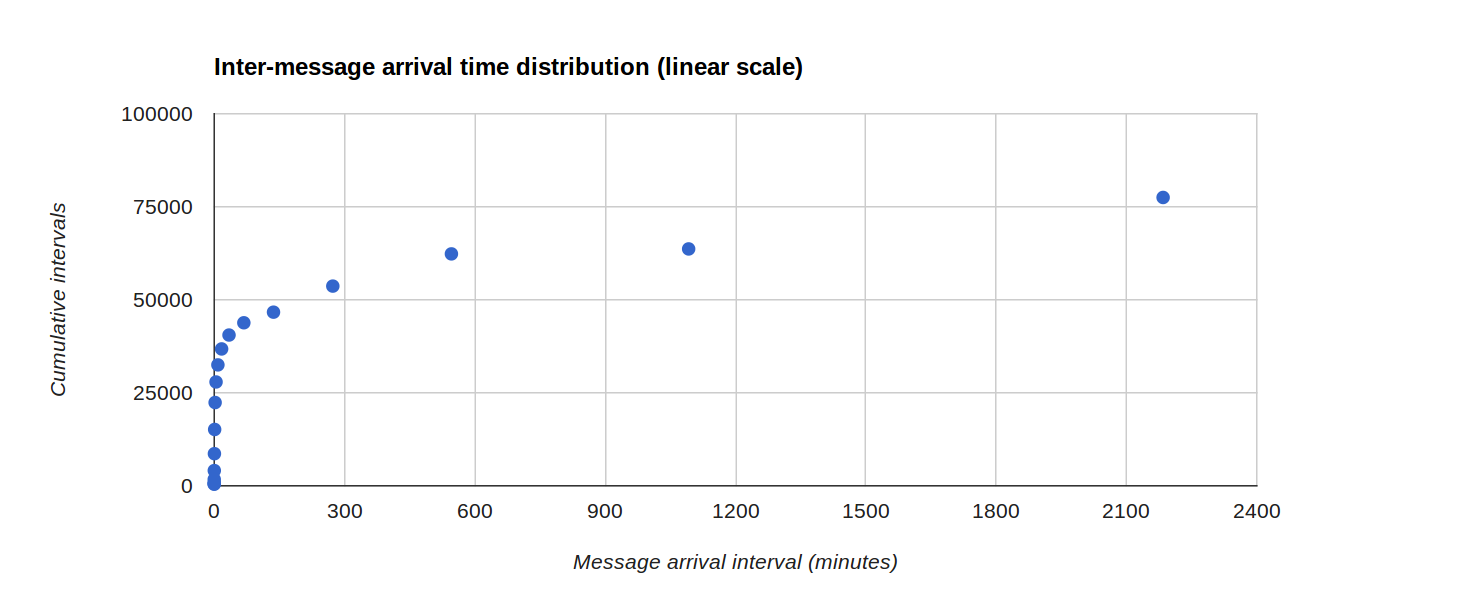
\includegraphics[width=\textwidth]{intermessagelinear}

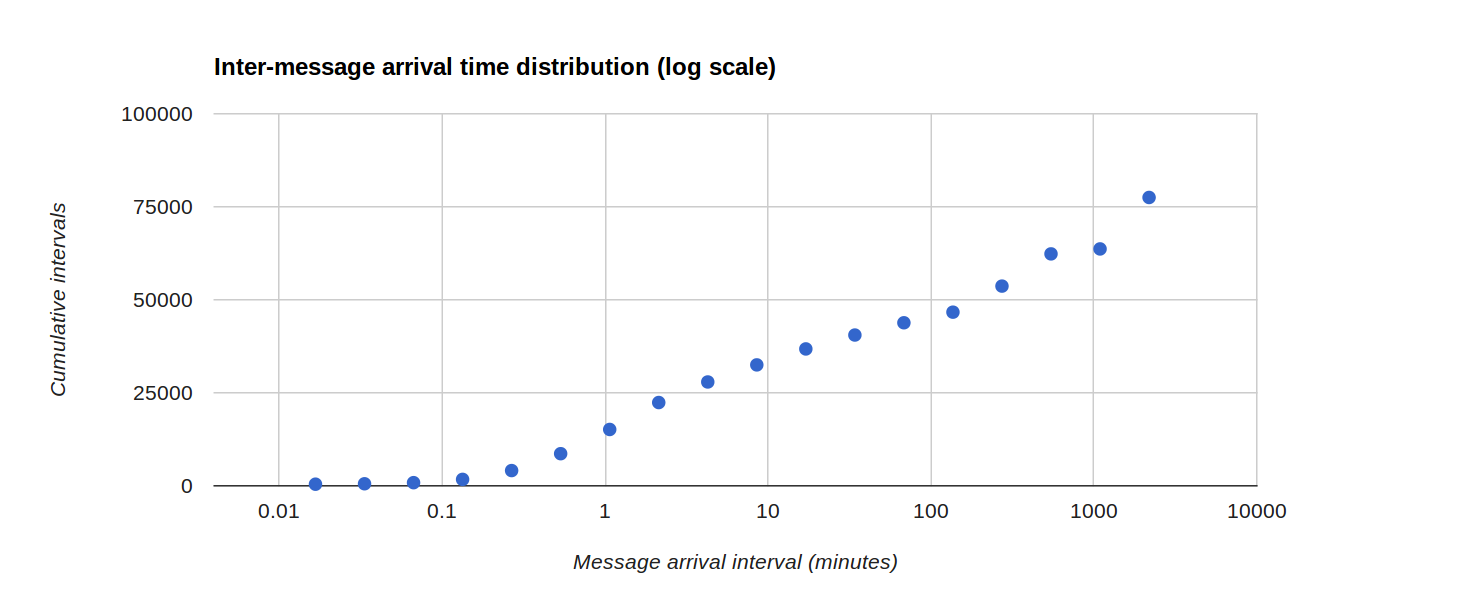
\includegraphics[width=\textwidth]{intermessagelog}


\section{Architecture and Data Flow}
\label{architecture}

% Have you defined your overall software architecture? -- describe it in detail and justify your design.

A permissible \project solution must be built to integrate with legacy systems. A metadata-secure client will also accept legacy SMTP traffic, and it must appear to the user that all messages, once received, are functionally the same. While the user experience must remain consistent, there are multiple possibilities for architecting a storage system consistent with the storage needs. To architect such a backend, there are several possibilities:

\begin{enumerate}
  \item Keep all messages on the local machine only.
    \item Store messages in a secure, remote, user-controlled filesystem.
    \item Use the infrastructure of existing IMAP servers.
\end{enumerate}

The first is unacceptable, given the target user group described in Section~\ref{targetuser}, as this would violate user expectations. Users expect to be able to access their content across all of their devices, and keeping all messages on the local machine only would thereby force them to adjust their usage patterns. To implement the second possibility, we would need to describe a server infrastructure for storing messages and synchronizing across multiple possible clients who have subscribed to updates on messages stored in the system -- which is to say, (a subset of) the functions that the IMAP server is designed to perform. This brings us to our final option: using a modified version of existing IMAP technology, as we have described.

In the \project protocol, a standard IMAP client library is wrapped with an \project module. A client then uses the \project module in lieu of a standard IMAP connection agent. The \project module will perform all necessary functions on behalf of the client, including encryption, message ID translation, and metadata tracking. The IMAP server is unmodified.
% The \project protocol is 
% The core elements of the \project protocol are 
% \begin{enumerate*}[label=(\itshape\arabic*\upshape)]
% \item an \project module used in lieu of a standard IMAP connection agent in an MUA, and
% \item an index file that is stored as a regular message in a legacy IMAP server. \end{enumerate*}
As further described in later sections, \project ensures that metadata is protected along with message contents for all messages to be stored on the IMAP server. It also handles the indexing functions, mapping pseudo-mailboxes to the messages they contain. This is a significant departure from the legacy system, where mailbox names and contents were exposed to the IMAP server. As such, it shifts the burden of tracking, updating, and syncing changes to the message metadata store (the INDEX) from the server to the client. When one client updates the INDEX, the IMAP server will receive the modified INDEX, making these changes visible to all other clients.

% Such updates may arise from moving messages between mailboxes as they appear to the client to exist, necessitating careful bookkeeping of the index file.

Note that these changes imply that if one client of an IMAP server is \projectnospace-compliant, all clients subscribed to that server must also be \projectnospace-compliant. Otherwise, all other clients will see only the encrypted messages as the IMAP server would see them; this is a necessary and desirable feature of the system.

These changes permit the combination of metadata-secure messages and non-metadata-secure messages in the same storage system, ensuring an elegant transition to a more secure email. While both types of messages can coexist under \project architecture, the pathways that they traverse to enter the system are distinct. In the next two subsections, we will discuss separately the receipt and insertion methods for messages received via legacy SMTP and for messages received from an alternative metadata-secure transport.

\subsection{Mail From a Secure Source}
\label{mail-from-secure}

When email is received from a metadata-free source (SMTorP, DIME, Pond, etc.), it is stored in a ``CRYPTOBLOBS'' mailbox on the IMAP server that the client's \project module has set up. This change is then marked in the INDEX, which is correspondingly updated.

  \begin{tikzpicture}[node distance=2.5cm]
  \node (alice) [box] {Alice};
  \node (smtpa) [box, above of=alice] {Alice's metadata-\\ secure server};
  \node (cloud) [cloud, draw,cloud puffs=10,cloud puff arc=120, aspect=2, inner ysep=1em, right of=smtpa, xshift=1.3cm] {Network};
  \node (imapb) [box, right of=cloud, xshift=1.3cm] {Bob's metadata-\\secure server};

  \node (bob) [box, below of=imapb] {Bob\\
  \trimbox{0cm 0cm 0cm -.2cm}{
  \begin{tikzpicture}
  \node (imaps) [box, minimum height=.5cm, outer sep=.2] {\project module};
  \end{tikzpicture}}};
  \node (bobimap) [box, right of=imapb, xshift=1cm] {Bob's legacy \\ IMAP server \\ \trimbox{0cm 0cm 0cm -.2cm}{
  \begin{tikzpicture}
  \node (index) [box, minimum height=.5cm, outer sep=.2] {INDEX};
  \end{tikzpicture}
  } };

  \draw [arrow] (alice) -- (smtpa);
  \draw [arrow] (smtpa) -- (cloud);
  \draw [arrow] (cloud) -- (imapb);
  \draw [arrow] (imapb) -- (bob);
  \draw [arrow] (bob) -| (bobimap);

  \end{tikzpicture}


\subsection{Mail From an Insecure Source}
\label{mail-from-insecure}

When an email is received through (legacy) SMTP, it is deleted from the server, its contents and metadata encrypted, and reuploaded to the IMAP server in the same way as an email that was received from a secure source.

  \begin{tikzpicture}[node distance=2.5cm]
  \node (alice) [box] {Alice};
  \node (smtpa) [box, above of=alice] {Alice's legacy \\ SMTP server};
  \node (cloud) [cloud, draw,cloud puffs=10,cloud puff arc=120, aspect=2, inner ysep=1em, right of=smtpa, xshift=1.3cm] {Network};
  \node (imapb) [box, minimum width = 4cm, right of=cloud, xshift=1.4cm] {Bob's legacy \\ IMAP server \\
      \trimbox{0cm 0cm 0cm -.2cm}{
          \begin{tikzpicture}
              \node (index) [box, minimum height=.5cm, outer sep=.2] {INDEX};
          \end{tikzpicture}
      } 
    };

  \node (bob) [box, minimum width = 4cm, below of=imapb] {Bob\\
    \trimbox{0cm 0cm 0cm -.2cm}{
    \begin{tikzpicture}
            \node (imaps) [box, minimum height=.5cm, outer sep=.2] {\project module};
        \end{tikzpicture}}};

  \draw [arrow] (alice) -- (smtpa);
  \draw [arrow] (smtpa) -- (cloud);
  \draw [arrow] (cloud) -- (imapb);
  \draw [arrow] (imapb.260) -- (bob.106);
  \draw [arrow] (bob.74) -- (imapb.280);

  \end{tikzpicture}
  
\section{Implementation Details}

Here we present the details of the system as it is currently implemented. While it currently implements only a subset of RFC 3501-specified functionality, it satisfies all requirements of Mailpile, its functioning client for prototyping purposes.

\subsection{Initialization}
\label{initialization}

Upon logging into an IMAP server, \project attempts to select the CRYPTOBLOBS mailbox. If it succeeds, it assumes that this server has been previously initialized by itself or another client. If there is no CRYPTOBLOBS mailbox, it creates one. It then generates a random salt, appends an initial INDEX with SEQUENCE NUMBER 1 and the salt in the subject line of the INDEX, appends a LOCK, and fetches and loads the INDEX.

\subsection{Command Translations}
In the IMAP server/client model, the client sends commands to the server, and the server responds based on its state and contents. These commands are the primary form of synchronizing data between the server and its clients. The \project module sits between the client and the legacy IMAP module. It translates arguments, processes data, and returns results that give the client a pseudo-view of the contents of the IMAP server informed by the contents of the metadata INDEX.

We can classify mailboxes by two features: their visibility to the server, and their visibility to the client. When the client's view of the mailbox is used, it is referred to as a pseudo-mailbox. There are four possible mailbox classifications, as illustrated in the table below. The classification determines the actions that the module takes in response to each command. A PSEUDO mailbox is not mirrored in the IMAP server; it exists only in the INDEX and is thus only known to clients following the \project protocol. SMTorP is an example of a PSEUDO mailbox. A HYBRID mailbox exists both in the IMAP server and in the INDEX. This is a mailbox such as INBOX, which must also be known to the IMAP server as a location for the delivery of incoming messages. A PSEUDO/HIDDEN pseudo-mailbox neither exists in the IMAP server nor is known to the client. It is only for the internal use of the \project module. The FAKE\_MESSAGES pseudo-mailbox used by the scheduler is an example of this type of pseudo-mailbox. An ACTUAL/HIDDEN mailbox is known to the IMAP server but not to the \project client. The CRYPTOBLOBS mailbox, the mailbox in which all encrypted messages are stored on the IMAP server, is an example of this type of mailbox. These classifications are shown in this table.

\begin{tabular}{ rr|c|c| }

 &\multicolumn{1}{r}{} & \multicolumn{2}{c}{Visible to Client?} \\

&\multicolumn{1}{r}{}
 &  \multicolumn{1}{c}{Yes}
 & \multicolumn{1}{c}{No} \\
\cline{3-4}
\multirow{2}{*}{Visible to Server?} & Yes & INBOX & CRYPTOBLOBS \\
\cline{3-4}
& No & SMTorP & FAKE\_MESSAGES \\
\cline{3-4}
\end{tabular}

\subsubsection{SELECT}
\label{select}

In a view of the system enforced by the Python wrapper for an IMAP connection, imaplib, when a SELECT command is passed to the IMAP module, the state of the IMAP server changes to record that a particular client connection has selected a mailbox, and returns a count of the number of messages in that mailbox. When the \project module receives a SELECT command, it saves the requested mailbox to an instance variable. If the requested mailbox is a HYBRID mailbox, it passes the count onto the IMAP server. For both PSEUDO and HYBRID mailboxes, \project then calculates the number of messages in the mailbox based on the INDEX, and adds that to either the returned value or 0. If a HIDDEN mailbox is requested, a NO response is returned. Note that the counting functionality is implemented by the EXISTS untagged request as further described in Section~\ref{exists} \---- the SELECT command additionally elicits the EXISTS server response, whose value is used for the return value of the Python function.

\subsubsection{FETCH} A FETCH or UID FETCH command requests information about a particular message, including either metadata or a subset of message body contents. For both metadata and body, \project first translates the requested permanent message ID (UID) as described in Section~\ref{uid-translation}. If it is a metadata request, it then forwards the translated command to the IMAP server, and forwards the response from the server. Note that metadata here means the metadata the IMAP server uses to keep track of its messages, namely FLAGS, INTERNALDATE, RFC822.SIZE, and ENVELOPE. If it is a body request, \project requests the entire message body (where body also includes headers). \project then checks that the hash matches, as further described in Section~\ref{rollback}. It then decrypts and checks the authentication of the message, as described in Section~\ref{encryption}. Finally, it returns the appropriate components as specified in the initial request.


Note that the present prototype implements only a subset of FETCH commands. Particularly, only metadata or the entire body can be requested. This is sufficient for use with the prototype's client, Mailpile.

\subsubsection{SEARCH} A SEARCH command acts on the selected mailbox. Similarly to SELECT handling as described in Section~\ref{select}, \project returns results from HYBRID and PSEUDO mailboxes as appropriate. The current version of the prototype only responds to SEARCH ALL commands, which list all UIDs in the mailbox in ascending order. By RFC 3501, the IMAP specification, a SEARCH command should handle a wide variety of requests. Many of these would require iterating through each message in the pseudo-mailbox, or searching on encrypted data. While one could imagine protocols for constructing efficient indexes or incorporating homomorphic encryption, such abilities are beyond the scope of this project.

\subsubsection{FLAGS} The FLAGS command is called for a specific mailbox, to ask which flags are valid inside that mailbox. Since the prototype client neither sets nor checks any message FLAGS itself, \project merely responds with the flags for the INBOX mailbox. A full implementation would allow flags to be set for individual messages within the metadata INDEX, largely reimplementing the IMAP server storage functionality on the client-side using the INDEX.

\subsubsection{UIDVALIDITY} UIDVALIDITY is a mechanism for detecting non-persistence of message UIDs. \project does not allow UIDs to change over time, so as per the RFC, we may return `1' for any mailbox where we are handling UIDs, pseudo or actual \cite{rfc3501}.

\subsubsection{EXISTS}
\label{exists}

EXISTS is functionally equivalent to the return value of SELECT. The technical definition is the number of messages in the mailbox.

\subsubsection{RECENT} RECENT is requested but ignored by the prototype client, so we return `0'.

\subsubsection{LIST} The LIST command is used to recursively find all mailboxes in the server. The current prototype allows only top-level, no-children PSEUDO mailboxes. Thus, in translating LIST results, \project inserts PSEUDO mailbox results as if existed at the top level. \project also removes HIDDEN mailboxes from the LIST results before returning.

\subsection{UID Storage and Lookup}
\label{uid-translation}

While all encrypted messages are stored on the IMAP server in the CRYPTOBLOBS mailbox, the client's view should allow for a more complex representation of which messages are stored in which mailboxes. At a minimum, we would like to support an INBOX mailbox for messages that are received at the IMAP server, and an SMTorP or Pond pseudo-mailbox for messages that are received at the client via a metadata-secure transport mechanism. Thus, each message needs an associated UID for its pseudo-mailbox, or the mailbox that the message is in as it appears to the client. But it also has an actual UID, or the UID inside the CRYPTOBLOBS mailbox (the server-view mailbox that stores all messages processed by \projectnospace). This UID is assigned by the IMAP server when \project APPENDs a message to a mailbox on the server. The APPEND command does not, however, return the assigned UID. Therefore we need a separate mechanism for associating a message's pseudo-UID with its actual UID.

To handle this, before appending a message to CRYPTOBLOBS, \project generates a 16-byte random UNIQUE SUBJECT number. This number is placed in the subject line of the appended message, forming a full subject line of the form ``ENCRYPTED <UNIQUE SUBJECT>''. Then, when the client requests a message via a specific mailbox/UID pair, \project uses the INDEX to look up the UNIQUE SUBJECT for the pseudo-UID in the appropriate pseudo-mailbox. It then searches for the message in CRYPTOBLOBS with UNIQUE SUBJECT in its subject line, which returns the unique actual UID of the message in the CRYPTOBLOBS mailbox.

For example, say the INDEX contains the following entry:

\begin{lstlisting}
INDEX = {`INBOX':{`36':`006a033f49f579f9a36e9afcfb1e7747'...}...}
\end{lstlisting}

If the client wished to acquire this message, it would issue the following commands:

\begin{lstlisting}
SELECT INBOX
UID FETCH 36 <REQUEST>
\end{lstlisting}

This would issue a request for message 36 in mailbox INBOX. \project would then note that
the UNIQUE SUBJECT for 36 in INBOX is 006a033f49f579f9a36e9afcfb1e7747, and issue the following requests to the server:

\begin{lstlisting}
SELECT CRYPTOBLOBS
SEARCH SUBJECT 006a033f49f579f9a36e9afcfb1e7747
\end{lstlisting}

This would return a list of all UIDs of messages with 006a033f49f579f9a36e9afcfb1e7747 as a substring of the subject in mailbox CRYPTOBLOBS. Since this is a 16-byte number, there is only a $1/2^{128}$ chance of two messages having the same UNIQUE SUBJECT, so this SEARCH will probably return only a single UID:

\begin{lstlisting}
OK 129
\end{lstlisting}


\projectnospace, now knowing the actual UID, can then issue the following request to the server:

\begin{lstlisting}
UID FETCH 129 <REQUEST>
\end{lstlisting}

One potential optimization here would be to perform the SEARCH immediately after each APPEND. The utility of this optimization is based on the number of subscribed clients and the probability of being selected to be pulled down in a mix. That is, if more than one FETCH will occur per APPEND, then it may make sense to cache the actual UID in the index.

\subsection{Processing Messages Received at the IMAP Server}
\label{processing}

When a message is received at the IMAP Server as in Section~\ref{mail-from-insecure}, \project processes the message so it bears surface equivalence to messages that arrived at the client machine from a secure source. Note that full equivalence can only be achieved by also including mixing steps either here or during scheduled message exchanges. Without them, it is trivial for an IMAP server to keep track of which message in CRYPTOBLOBS corresponds to which message that was received in the INBOX, because the server will see that a message was added to CRYPTOBLOBS and deleted from INBOX at about the same time.

To process a message, \project fetches the body of the message, adds it to CRYPTOBLOBS, and deletes it from the INBOX. The process used for adding the message to CRYPTOBLOBS is equivalent to the process for adding a message from an insecure source, or for adding a scheduled fake message. The process for adding a message to a pseudo-mailbox involves several steps. We update the INDEX, possibly adding the mailbox to the INDEX if it is the first time we have seen it. We generate a UNIQUE SUBJECT number. If the mailbox is of type PSEUDO, we compute the pseudo-UID for the message. As per RFC 3501, the UID assigned is strictly greater than any UID that has been previously assigned in the mailbox. We store in the INDEX the state of the NEXT UID to assign.


\subsection{Multiple Client Synchronization and Concurrency}
Central to IMAP's design is the ability to handle the actions of multiple clients subscribed to the server. The core synchronization feature is the INDEX. Since it resides in the CRYPTOBLOBS folder that all IMAP clients have access to, any client will see the updates to the INDEX made by any other client. Some actions need only be completed by one client though, such as those described in Sections~\ref{initialization} and \ref{processing}. These will be handled by the first client to notice the preconditions for those actions, namely an uninitialized IMAP server or a message in the actual INBOX mailbox.

Given the structure of the IMAP commands, there is no drawback to being either the first or a later client to perform the action. For example, a client of \project that asks how many messages are in the INBOX will be returned the same number in response to a SELECT whether they were the one to process an incoming message or not, and will be returned the same list of pseudo-UIDs in response to a SEARCH ALL.

Some \project actions must be atomic, namely the coupling of appending and deleting messages from mailboxes with fetches of and updates to the INDEX. \project solves this via a LOCK mechanism. A message with SUBJECT line LOCK is deleted from and appended to the CRYPTOBLOBS mailbox to acquire and release a lock, respectively.

Because of this delete/upload lock acquisition mechanism, the IMAP server may sometimes be in a state where the LOCK message does not exist but no client holds the lock, such as if a client crashes or closes down while holding the lock. Optimally, this would not happen, and the lock would be released before closing. Unfortunately, the existing library (imaplib) allows its client to close its socket directly, rather than through a specified method at the library level, so we cannot rely on a client to release a lock before quitting. Thus, \project includes a mechanism for detecting this inconsistent state and recovering from it by acquiring a lock even if the LOCK message does not exist in the CRYPTOBLOBS mailbox.

The lock recovery mechanism waits until a specified time (default 60 seconds), checking for the existence of the lock every few (default 2) seconds within that interval. After the time is completed, \project attempts to fetch the INDEX. If the index is not there, we assume that another client has experienced a failure and acquire the lock ourselves. If the index is there but has not been updated during that time (using its SEQUENCE NUMBER to determine this), we again acquire the lock. Yet if the index is there and has been updated, we assume someone else is still using the lock and double the total wait time until our next check. This mechanism could create a race condition in re-creating a lost LOCK, when multiple waiting clients fulfil their LOCK re-acquisition conditions simultaneously and therefore both attempt to take the LOCK themselves. We could address this in various manners. \project could decouple LOCK acquisition and recovery mechanisms, or partially decouple them by recreating a lost LOCK, waiting, then acquiring it. Additionally, \project could mitigate simultaneity by waiting a randomized time selected from an exponential distribution before acquiring a lost LOCK, so that multiple waiting clients are less likely to do simultaneous re-creations.

\subsection{Deletion}
Various \project actions involve deletion of a message from the CRYPTOBLOBS mailbox. In general, not deleting a message will not leak any data to the IMAP server, since our threat model includes a server than can either refuse to delete or can save a backup version of any message. Yet for practical reasons such as server data usage and lack of clutter, it is generally beneficial to at least allow a client to attempt to delete a message. Here we must note that IMAP servers may differ in their implementation in regard to the location of messages, potentially complicating deletion protocols. For example, Gmail uses its All Mail mailbox (``label'', in their terms) as a message archive \cite{allmail}. That is, if a message appears in any mailbox, it will also appear in the All Mail mailbox. If it is deleted from All Mail but still exists elsewhere, it will be replaced in All Mail. Thus, to delete a message from any non-All Mail mailbox, it must first be deleted from all other mailboxes then deleted from All Mail. Note that the message will be assigned a different UID for each mailbox that it appears in.

Deleting a message that has already been processed is simple; we may use UNIQUE SUBJECT as in Section~\ref{uid-translation} to find the message in any mailbox, including All Mail. For a message that has arrived in the INBOX though, we must be more careful. To delete such a message from All Mail, we must first search for it (by subject or otherwise), then test all resulting UIDs for exact message equivalence to the message that we intend to delete from the non-All Mail mailbox.

\subsection{INDEX Caching}
From the perspective of the \project module being used as a general system library, each individual command that requires access to the INDEX should re-fetch it before executing the command, in case the INDEX has since been changed by another client. (This is different from operations requiring the LOCK, which is used for making multiple calls atomic.) Yet from a practical perspective, this can slow down the program immensely, since certain calls are often executed in batches and are tightly coupled. For example, our prototype client calls the RESPONSE command with an argument of FLAGS, RECENT, UIDVALIDITY, and EXISTS in quick succession. This is an artifact of the translation into a Python library, since these are sent by the server in response to a SELECT command, but their results (except for the count returned by EXISTS) are not included in the library command's return value for a SEARCH request. To handle this overfetching, it might be reasonable to alter the method signature of certain commands in the \project library to allow a flag indicating that it is acceptable to consult a cached version of the INDEX. For example, a client might choose to request an uncached INDEX for the first in a series of commands sent to check all mailboxes for new messages, but allow a cached INDEX for subsequent mailbox requests, and only begin requesting the INDEX again if there are in fact new messages available to fetch.

\subsection{Prototype Client}
In this implementation, we integrated \project with Mailpile, an open source mail client implemented in Python that includes an SMTorP plugin. Mailpile is a webmail client that is able to run either locally or on a trusted server, where it can be accessed from any browser. Mailpile multiplexes all IMAP commands over a single open connection, and not all threads have access to the open connection. This means that calls to the \project module where connections will be made to the server must be called from the appropriate thread. For example, when sending a message that arrived over SMTorP, the message can be cached locally from any thread, but the thread that calls the timer tick method to send it on schedule must have previously opened a connection and logged in. Mailpile also requires the user to provide a passphrase to unlock the data stored locally. This passphrase could be forwarded to the \project module as the passphrase for encryption, or Mailpile could ask for a separate passphrase. While the current \project implementation takes a passphrase in the constructor, any key would technically work, if the client chose to derive a key from the passphrase and handle key management itself.

In the course of this project, three bugs were found in the Mailpile implementation (for one of these, a pull request has been submitted and accepted), indicating that for full security assurance, a more developed client should likely be used.




\section{Security}

In addition to metadata security, \project conforms to standard expectations of a secure system.


\subsection{Encryption}
\label{encryption}

When a message is appended to the CRYPTOBLOBS mailbox, whether it be a processed INBOX message, a fake message created on schedule, or a message from a metadata-secure source, it is encrypted before being uploaded. It is encrypted using the standard method of authenticated encryption, which is to say that a Message Authentication Code computed on the encrypted message is concatenated to the encrypted message. Data is encrypted using AES-CBC and signed with HMAC-SHA256. The encryption key is derived from the random salt created during initialization (as described in Section~\ref{initialization}) and a passphrase using scrypt \cite{percival2009stronger}. Scrypt is a memory-hard key derivation function that imposes a cost for deriving a key given a guess of a passphrase by using many sequential iterations that cannot be parallelized on specialized hardware.

The passphrase is passed into the \project module at runtime initialization of the class. This leaves handling of the passphrase to the client. The client can choose to ask the user for it on each initialization, ask once and save for future use, or a hybrid of the two methods. The user can choose a passphrase, or the client can generate a passphrase and instruct the user to save it. The latter method is currently not supported (although it could be), as it would require a mechanism for merely checking if the server has been initialized without initializing it. If the programmatically-generated passphrase method is used, we suggest displaying it to the user as a ``backup code'' as in Yahoo!'s End-to-End Encryption Extension \cite{yahoo} for usability reasons; users are familiar with the concept of backing up data, but may not be as familiar with keys and passphrases.


\subsection{Rollback Detection}
\label{rollback}

While we cannot rely on the IMAP server for availability, we can detect and decline to accept rollback of any part of the system. In a rollback attack, an adversary in control of the server can partially or completely snapshot the files on the server at any given time, then later replace a file with that name with its old contents. So, if the server took a snapshot of one version of the INDEX, then a client changed the INDEX to reflect deletion of a message, the server could later replace the current INDEX with the previous one, making it appear as though the message had not been deleted. This would be particularly problematic if a unique subject is reused, which could cause a client to receive a different message for that subject than they should have seen.

To address this, we employ a rollback detection mechanism. Each time that the INDEX is updated by any client, its SEQUENCE NUMBER is incremented. Thus, when a new INDEX is downloaded, the \project module compares the SEQUENCE NUMBER of the received INDEX to the most recent SEQUENCE NUMBER it has seen. If the downloaded sequence number is not at least the value of the SEQUENCE NUMBER known to the client, then the new index is not accepted. It saves this value in memory, but also stores it to a local file specified by the client of the module. When a client connects to an IMAP server that has already been initialized for the first time, it uses the current INDEX's SEQUENCE NUMBER as the initial number.

Rollback detection for individual messages relies on the rollback detection of the INDEX. When a message is appended to CRYPTOBLOBS, its hash is saved in the INDEX along with its pseudo-UID and UNIQUE SUBJECT. Each time the message body is FETCHed, the body is hashed and compared to the saved hash. If they differ, then the message has been changed. Thus, assuming a current INDEX and knowing that the INDEX is saved in the server under authenticated encryption, an adversary cannot replace the message with a version whose hash is not saved in the current INDEX.


\section{Protecting Metadata}
Once a message has been received at the client, we would like to upload it to the IMAP server for storage. Yet while we can hide the FROM and TO headers easily, we do not want the server to gain timing information about the message. If we upload it immediately, then the server will know that we have received a message at that time. Even worse, modern clients often save sent messages to a Sent Messages mailbox. If the mail server of the sender and the receiver are colluding, as can easily be the case when both clients are using the same company to provide servers, then the server could easily execute timing attacks by observing two users suspected to be communicating, and seeing if they upload a message at about the same time. So, we must include a mechanism for hiding this timing metadata from the IMAP server. The solution must not:

\begin{itemize}
  \item allow the server to recover the timing information,
  \item take up an extraneous amount of space in the mailbox, or
  \item reveal otherwise hidden information via the deletion of a message.
\end{itemize}

Yet even under these constraints, it must allow sufficiently frequent and short exchanges with the server.


\subsection{Mechanisms}
While we can vary particular parameters and algorithms, most potential solutions discussed in this section rely on two primary components, scheduling and mixing. By scheduling, we mean that the client will exchange data with the server on a set or randomized schedule. By mixing, we mean that in an exchange with the server, multiple messages will be deleted, and multiple messages uploaded in their place, with only the client being aware of the correlations between messages deleted and uploaded.

  \begin{tikzpicture}[node distance=8cm]
  \node (\project) [box, minimum height=2cm] {\project};

  \node (scheduler) [box, minimum height=2cm, right of=\project] {Scheduler};

  \draw [arrow] (\project.10) -- node [above] {State information} (scheduler.-190);
  \draw [arrow] (scheduler.190) -- node [below] {Next action type} (\project.-10);
 
  \end{tikzpicture}

Fundamentally, scheduling means that \project performs an action at a predetermined time tick. To better reason about the leakage of information, \project contains a separate scheduler module (shown above) that is informed when a message arrives or is marked for deletion. This scheduler can thus reason about the expansion rate of the server. At the scheduled time tick, \project will ask the scheduler what its next action should be. This can be one of three types: UP, DOWN, or NONE. UP means that the server will grow in size by one message, DOWN means that it will shrink by one message, and NONE means that the total server size will remain constant. The ternary digit (trit) that it outputs is based on its metadata protection policy, determined in conjunction with the \project module. We separate this functionality into the scheduler because it precisely mirrors the information that the server will receive: whether a message has been pushed up, pulled down, or neither. Thus, the server can gain no more than one trit of data on every time tick.

To implement this one-trit leakage, \project must perform the determined action on each timer tick, whether or not it is has a message to deliver or a deletion scheduled. This condition is satisfied through artificially constructed messages. A constructed message with contents of a random size chosen from a distribution mirroring that of messages usually sent and received by the user is generated, encrypted and packaged as if it were a legitimate message, saved to a FAKE MESSAGES pseudo-mailbox, and sent to the server. On deletion, a message from FAKE MESSAGES is chosen at random and deleted in lieu of a legitimate message. Without taking into account any other information, these actions would appear identical to the server whether they were performed on real or fake messages, since the server will see only updates to the INDEX and the append or delete of a message with subject ENCRYPTED <UNIQUE SUBJECT> and encrypted contents. How they appear to the server in the context of all actions taken by \project together is the subject of Section~\ref{best-metadata}.

\project also incorporates mixing to better hide metadata. In a single mixing step, MIX NUMBER messages are fetched and deleted from the server, and MIX NUMBER $\pm 1$ messages are pushed back to the server so that a particular message in the former set can be associated with all messages in the latter set with equal probability. Note that for mixing to be effective, all messages included in the mix must be of the same size. Which messages are selected to be a part of the mix depends on the metadata hiding strategy.


\subsection{Strategies}
\label{best-metadata}

To provide metadata security, we must carefully apply scheduling and mixing in our communications with the IMAP server. The requirements that \project has for operations on messages bear resemblance to those of memory operations in oblivious random access memory (ORAM)\cite{oram}. ORAM assumes a situation where multiple actors (say CPUs) can see memory access and store actions on a shared memory module. It proposes a system of additional memory accesses and locations to shield patterns of which memory locations have been accessed, making read and write operations indistinguishable from each other. ORAM techniques and implementations are an active area of research, some with proven lower bounds on additional bandwidth cost \cite{stefanov2013path}.

ORAM makes assumptions that we could perhaps consider relaxing. First, ORAM assumes constant, fixed-size blocks of memory. Messages in a mail server need not be constant size, although any solution that involves mixing will require elements of the mix to all be of the same size. Second, a primary goal of ORAM is to hide correlated memory locations; that is, memory locations that are often accessed together and might therefore reveal information about the structure of the program or the data. We could theoretically restrict ourselves from the full scope of desirable actions, such as by choosing not to decompose messages into fixed-size chunks and saving all messages into the same pseudo-mailbox. Were we to do so, then an individual message will not be inherently correlated with any other message. Note that mixing will generally require chunking of messages, and we wish to support multiple pseudo-mailboxes, but locations are not as inherently correlated in all cases as they are when a program is executing on memory locations. Third, mailboxes do not allow store operations in the sense of RAM; IMAP only supports appending to mailboxes. Even under these relaxations, we will see that most solutions that do not implement an ORAM-adherent technique will trade off either functionality or security.


\subsubsection{Scheduling, no mixing}
Could we implement a mix-free solution where we only schedule UP and DOWN operations, hiding actual message additions and deletions among many fake ones? In such a situation, future actions ideally should not reveal information about which messages previously pushed were real and which were fake. Particularly, assuming that deletions of fake messages occur much more frequently than deletions of real messages, deletion operations should reveal neither whether the particular message deleted or any other was real. Additionally, message fetches must similarly not reveal information regarding the veracity of that message or any other. Note that this last restriction immediately disqualifies this solution barring additional mechanisms to mask message fetches by any client of the server that attempts to download all real messages. Further, naive fetches would leak information about which messages are grouped together in a single mailbox. We will see that it is not practical to attempt to find such mechanisms, since the rate of growth required to sufficiently mask deletion operations is infeasible.

Consider the trivially incorrect case where server growth roughly mirrors the rate of incoming real messages. We upload two messages to the server, R and F. R is a real message, and F a fake. Initially, the server cannot distinguish between the two messages. Since R is real, there is some user-dependent probability $p$ that it will be deleted at any point in the future. Given the availability of storage, a modern trend of archiving, and that these messages are encrypted, we can assume that $p$ is very small. Since we are looking to have server growth mirror the rate of incoming real messages, the goal of the scheduling algorithm is to send messages to the server at an effective rate similar to the rate of actual message receipt, so the server does not grow needlessly. Then, the number of fake messages will remain about constant, $k$. So at each timer tick where a DOWN occurs, a fake message will have probability $p=1/k$ of being deleted. Therefore, the probability that a message is not deleted after $n$ DOWN ticks is $(1-1/k)^n$ (since it must not be deleted at all time ticks), which tends towards 0 as $n$ increases. Thus, a fake message's long-term probability of being deleted is 1. So, after a length of time has passed, any message that was uploaded to the server and has remained there for a long period of time is likely a real message, and the server can therefore merely observe the time it was uploaded.

This analysis does not only apply in the theoretical sense. Assume the user had let the system run in a mode where more fake messages are uploaded than are deleted until it was seeded with 5,000 fake messages. After that point, the user wants to keep the size of the mailbox constant, so for each upload (received message), they delete a message as well. Assume also that they would like to spread new messages to other clients of the server within 10 minutes of its receipt (a conservative estimate). Then they must delete a message every 10 minutes as well, which amounts to 144 deletions a day, 52,560 a year, and 262,800 in a five year period, which we conservatively assume is the length of time a user would like to keep an email account for. So $k=5000$ and $n=262800$, giving a probability of a fake message not being deleted of about $1.5\times10^{-23}$, which is certainly distinguishable from $1-p \approx 1$ for a real message.

Now assume instead that we will let the server grow to some extent. By adding more fake messages than real messages, we will drive down the probability that a fake message is chosen for deletion until it resembles the probability that a real message is chosen. How often could we delete messages chosen from the set of all fake messages at random before we lose the ability to hide real messages among the fake ones? Assume for simplicity that fake messages are added at an amortized constant rate. We would like to calculate the probability that a fake message is not deleted after the $n$ DOWN ticks following its upload at time $t$. This is equal to the product of the probabilities that a fake message was not deleted at all ticks between times $t$ and $t+n$. We can compute this based on the probability of deleting a message at a particular time after $i$ deletion intervals. Assume that at each each interval, $c+1$ real messages and $f$ fake messages came in. Then the probability that a message was fake is $f/(c+f+1)$, and $c+f+1$ messages total came in each interval. But one message was deleted each interval, so $c+f$ net messages are added. So after $i$ intervals, $i(c+f)$ total messages are in the server, and an expected $i(c+f)f/(c+f+1)\approx if$ of those are fake. So the probability of a message being deleted at time $i$ given that it is fake is $1/(if)$, and the probability that it is not deleted is $1-1/(if)$. Then if the message was uploaded at time $t$, the probability that it was not deleted at time $n$ is $\displaystyle\prod_{i=t}^{i=t+n}(1-\frac{1}{if})$. This product tends towards 0 as $n$ tends towards infinity, but its slope drops off quickly as $f$ increases.

For example, consider the following graph of the probability of a message being not deleted from when it was added at time $i=250$, until time $i=1000$.

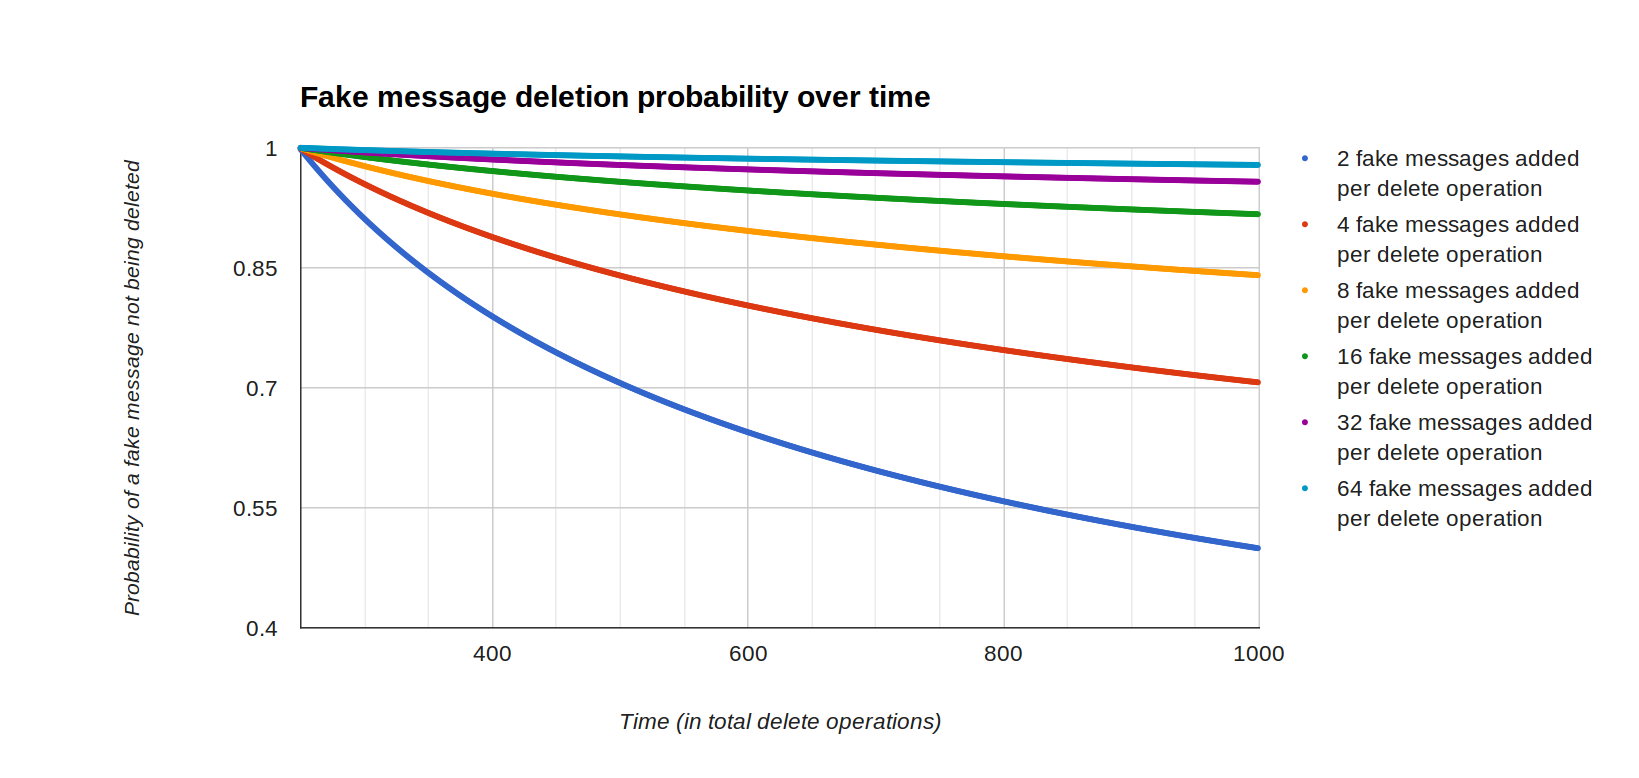
\includegraphics[width=\textwidth]{many_lines_2}

Note that if 32 or 64 messages are added per deletion operation, the probability that a fake message is not deleted remains at 0.96 and 0.98 respectively even after $1000-250=750$ operations. This comparison is shown more clearly in the following graph, where we see that for high numbers of messages added per delete operation, we maintain high probabilities of fake message not being deleted, as the probability varies near-logarithmically with the number of fake messages added.

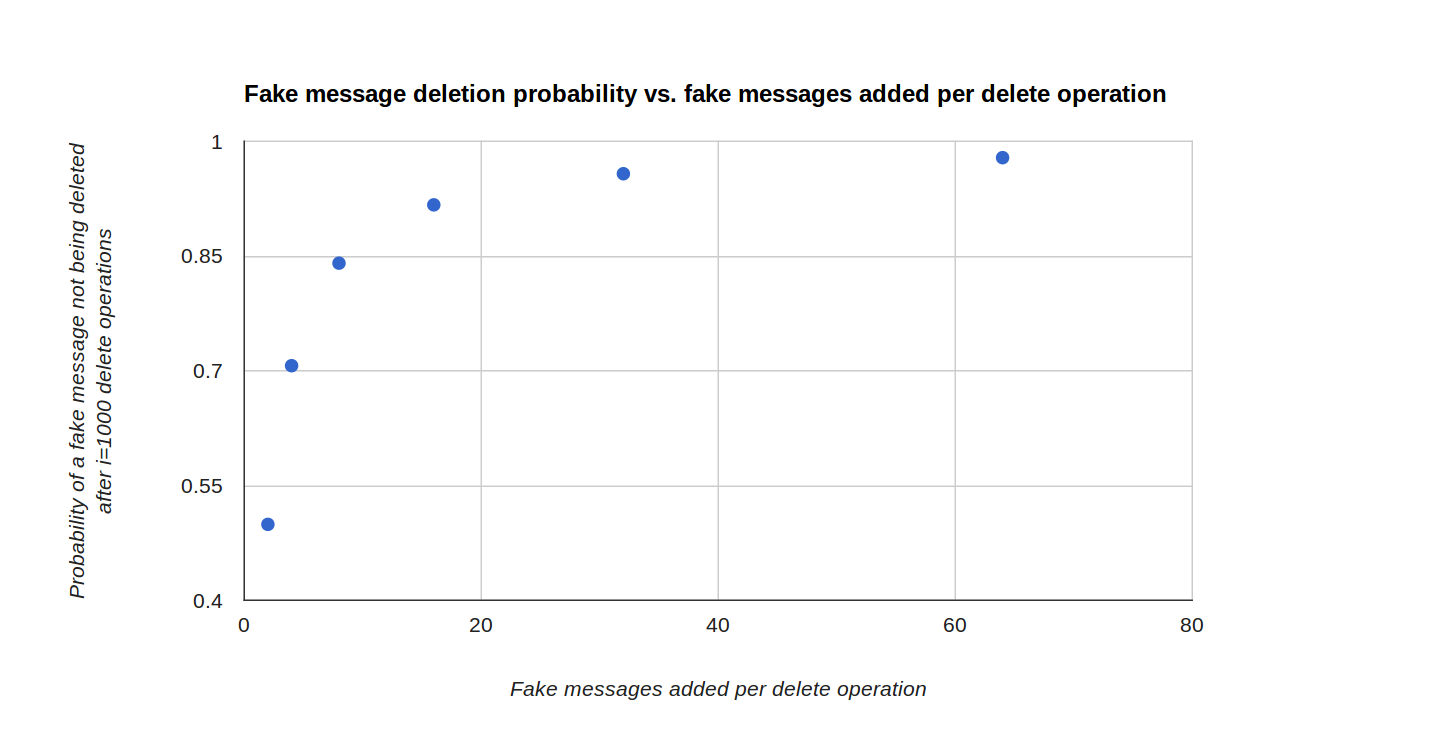
\includegraphics[width=\textwidth]{few-blue-dots-250}


Yet we only achieve these high rates after the server has been seeded with an adequate number of fake messages, as demonstrated by altering our parameters to show the results when a fake message is instead added at interval $i=0$.

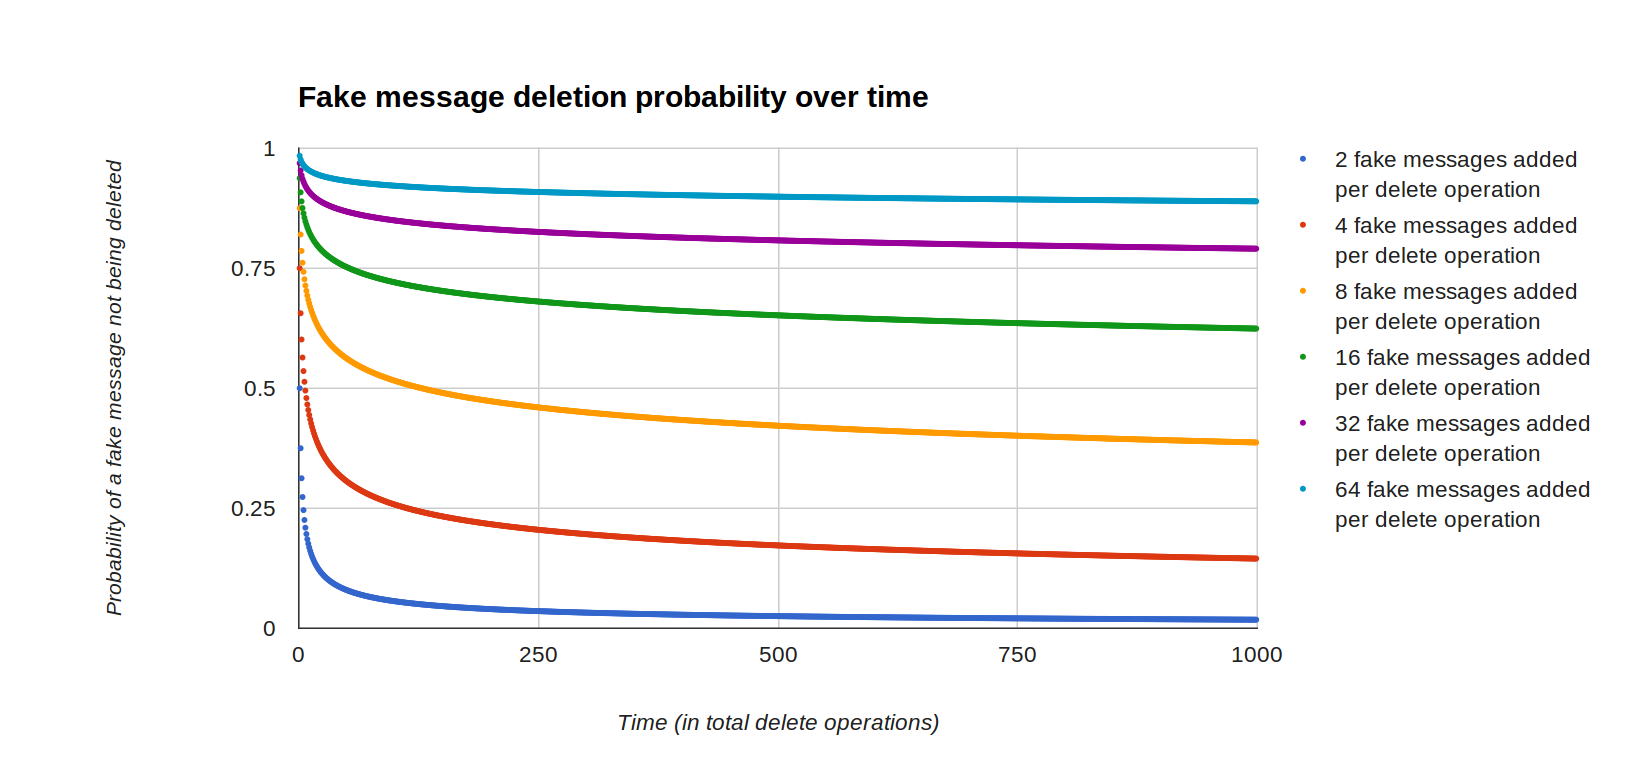
\includegraphics[width=\textwidth]{fake-message-deletion-over-time}

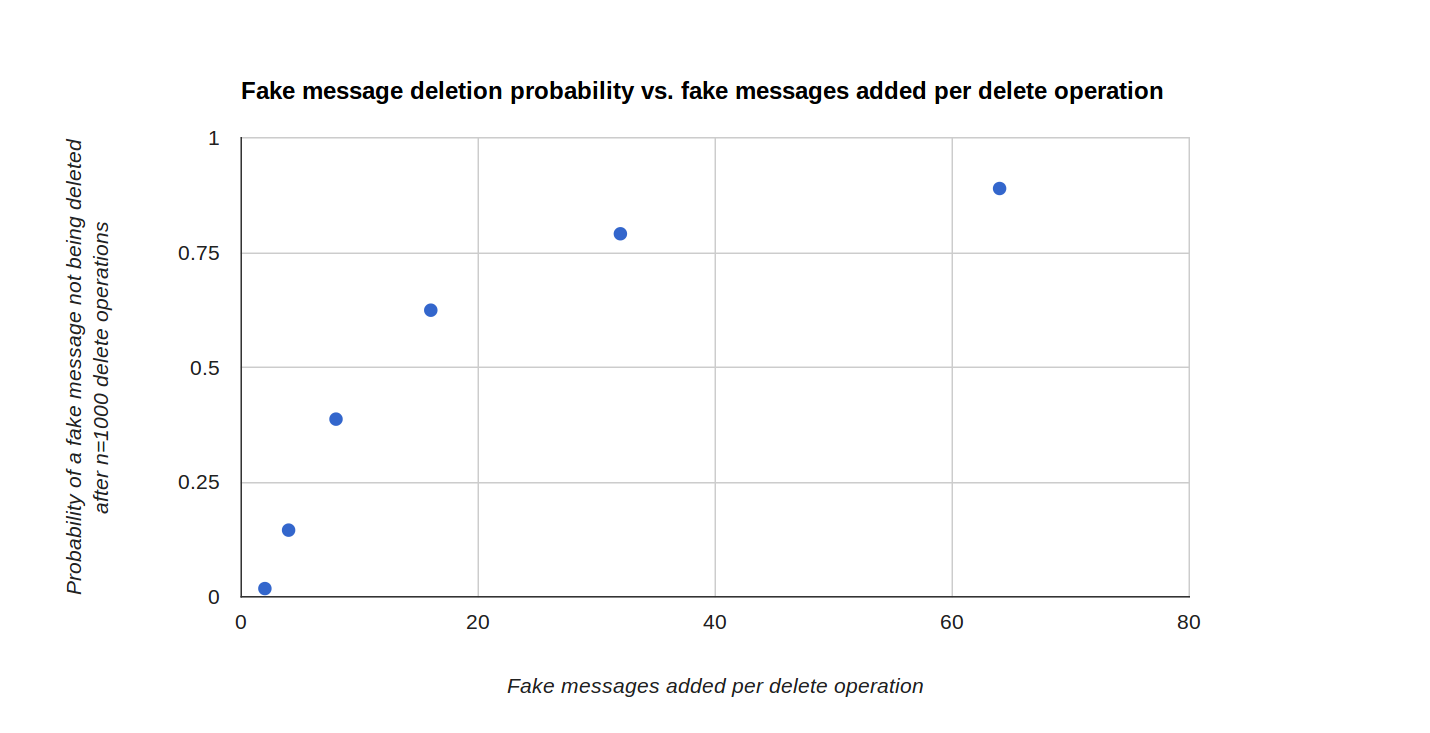
\includegraphics[width=\textwidth]{fake-message-deletion-probability-vs-num-fake-messages-added}

In this case, we need an $f$ of 64 to achieve merely a $p=0.89$ that a fake message is not deleted (compare, of course, with $p \approx 1$ for a real message under the assumption that few real messages are ever deleted). Thus, to achieve even a relatively feasible probability match, we could delete only 1 in 64 messages.

Is this rate of growth sustainable? Theoretically it is, of course, but not given reasonable expectations of server longevity. Assume we would like to delete a message every 64 messages that were pushed, and that one operation occurs per time tick. The following graph relates message check frequency for varying numbers of clients connected to an IMAP server with time to fill a mailbox. The total mailbox size is Gmail's current size of 17 GB, with an average message size of 170 kB.

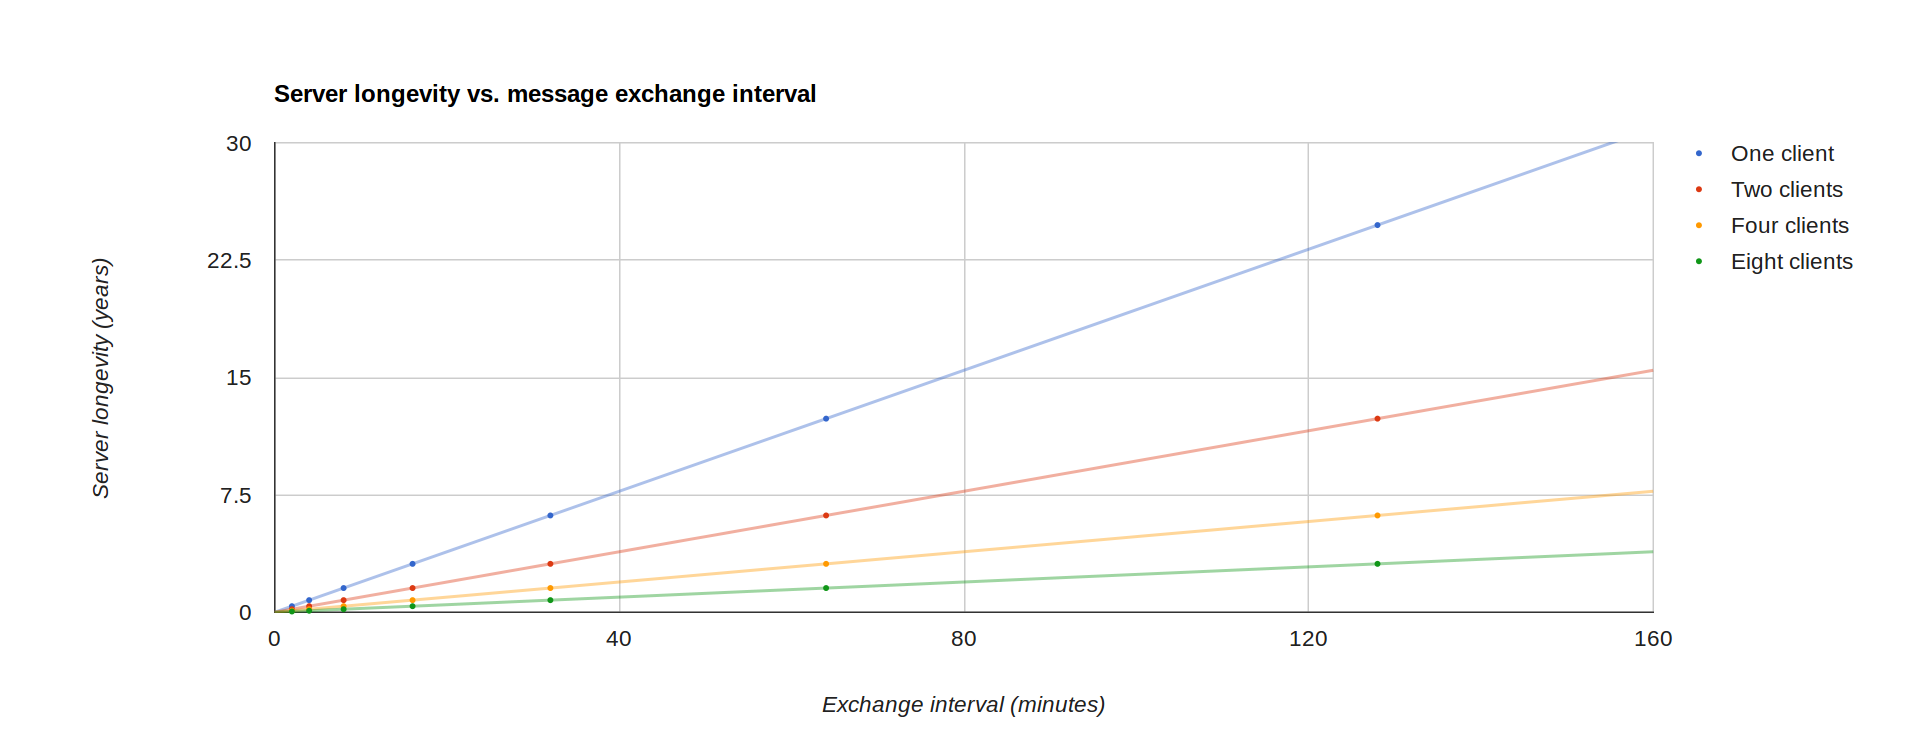
\includegraphics[width=\textwidth]{server_longevity}

With only two clients, if we wish to check our mail more than once every half hour (both of which are conservative estimates), we would use up the entire alloted space in three years. To compensate for space costs, we can introduce mixing operations.

\subsubsection{Mixing with \texorpdfstring{$O(1)$}{O(1)} decoys}

If we wish the growth rate of the server to precisely match the rate of messages to be pushed, we could consider performing many mixing operations. Intuitively, this could work because to grow with the actual rate, each fake message that was in an UP operation (a scheduled exchange with the server where one more message is sent to the server than is deleted from the server) must appear in a DOWN operation (a scheduled exchange with the server where one fewer message is sent to the server than is deleted from the server). Mathematically, assume that the mailbox is seeded with $k-1$ fake messages. Consider again messages R and F, and call MIX NUMBER $m$. This time, R and F were each one of $m + 1$ messages pushed to the server, with R pushed into set A and F pushed into set B. Assume no overlap between A and B, since $m<<n$, the total number of messages. This case is similar to the case of no extraneous growth without mixing assessed above, since we are extremely unlikely to have selected a message in set B for inclusion in the mix were one of them not fake. More precisely, we have at least a $1/k$ probability of choosing a message from set B. For choosing at least one message from set A, though, we have a probability equivalent to $1-q$, where $q$ is the probability of choosing 0 messages from set A. The probability of $q$ can be computed, since it is equivalent to choosing all $m$ messages from the $n-m$ messages not in set A, which there are ${{n-m}\choose m}$ ways to do. This gives a probability of choosing at least one message of the $m$ chosen messages from set A of $1-\frac{{{n-m}\choose m}}{{n \choose m}}$.

For a reasonable estimation, assume $n=5000$ and $m=10$, which gives a probability of choosing from set A of slightly under 0.02. Then, $k$ must be at least 50 to give equivalent probabilities for choosing from sets A and B. But this analysis only applies if the adversary does not know which of the messages are the fake $k$ at every time step. So, how many mixing operations do we require to completely mix all $n$ messages? If we are selecting at random, this is the expected number of operations required to select all $n$ messages in batches of $m$, which is a variation on the coupon collector problem. It is not precisely the coupon collector problem, since we are selecting $m$ at a time, and therefore one batch cannot contain duplicates of the same message, so there is a slightly higher probability of selecting a never before seen message for later messages in a batch. Thus, we can place a lower bound on the number of mixing operations required to select $n$ messages at $E(n) = n \ln (n) / m$. Using our estimates of $5000$ and 10, this is over 4000 mixing operations. We must pull down and push up a total of $2m$ messages for each operation, so that is $2n\ln (n)$ messages that must be transferred to entirely mix the mailbox regardless of $m$. This is unreasonable to do on a regular basis.


\subsubsection{Mixing with \texorpdfstring{$f(n)$}{f(n)} decoys}
\label{fofn}
With more decoy messages, we could select messages for mixing at random, thereby avoiding issues of distingushing between real and fake messages based on probabilistic distinctions. That is, we could initially seed the server with $f(n)$ messages, and schedule only NONE mixing operations where additional messages appear to neither be pulled nor pushed to the server. Then, when a fake message is randomly selected to appear in the set of messages to be mixed and there is a real message queued for upload to the server, the real message will opportunistically take the place of the fake message in the mix. Likewise, when a real message is selected for deletion, it will be silently replaced with a fake message. The scheduler will then separately decide when to insert an additional fake message in a mix. This insertion is based only on the number of total messages in the server, which the server itself can observe, so no data is leaked there, either.

What does $f(n)$ need to be to ensure a reasonable rate of selecting a fake message? Again assuming a batch size of $m$, we can compute the probability that a fake message is included in a batch, and thereby compute the expected number of mixes before including a fake message in a batch. Here again we can trade off between $f(n)$ (which determines total server size), $m$ (which determines bandwidth and speed), and frequency of mixes to achieve equivalent rates of being able to insert a message.

The following graphs show, for various functions of $n$, the expected number of mixes before including a fake message in a mixing batch vs. values of $n$, given different batch sizes $m$. To calculate the graphed values, we find the expected number of mixes before encountering a fake message, given that each mix has a probability $p$ of including at least one fake message. Since mixes have independent probability of encountering a fake message, this expected value is $1/p$. To calculate $p$, we consider that we are choosing $m$ messages from a total size of $n$, and we would like the probability of selecting at least one fake message given that there are $k=f(n)$ fake messages. This is equivalent to $1-q$, where $q$ is again the probability of choosing 0 fake messages, or $\frac{{{n-k}\choose m}}{{n \choose m}}$.

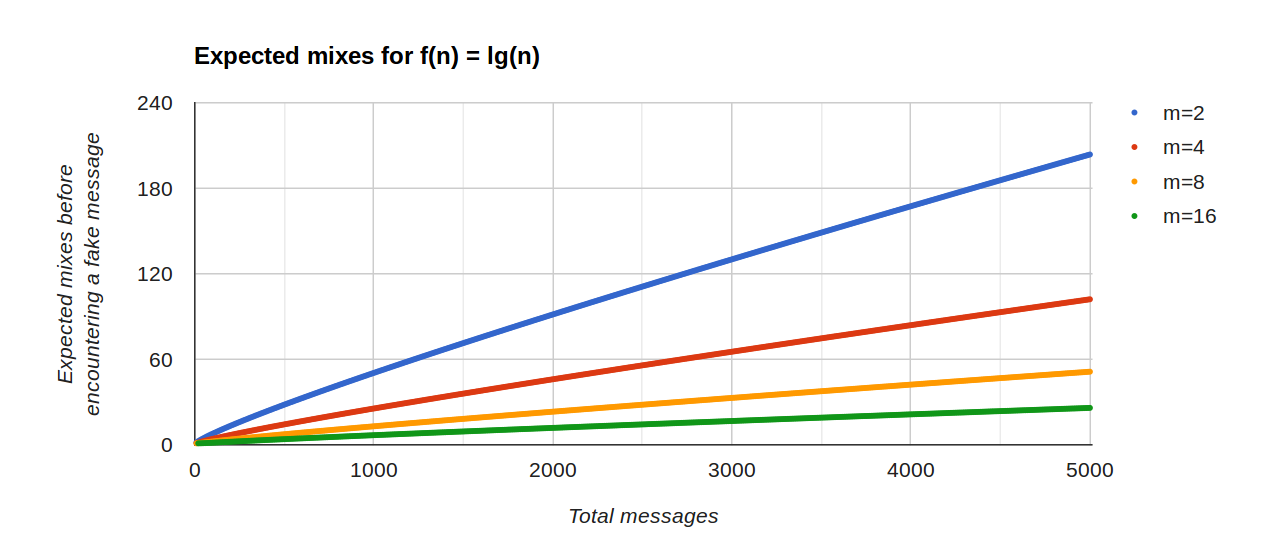
\includegraphics[width=\textwidth]{lgn}

Using the logarithm base 2 of $n$ causes the number of fake messages to grow too slowly relative to $n$ to achieve sufficient saturation.

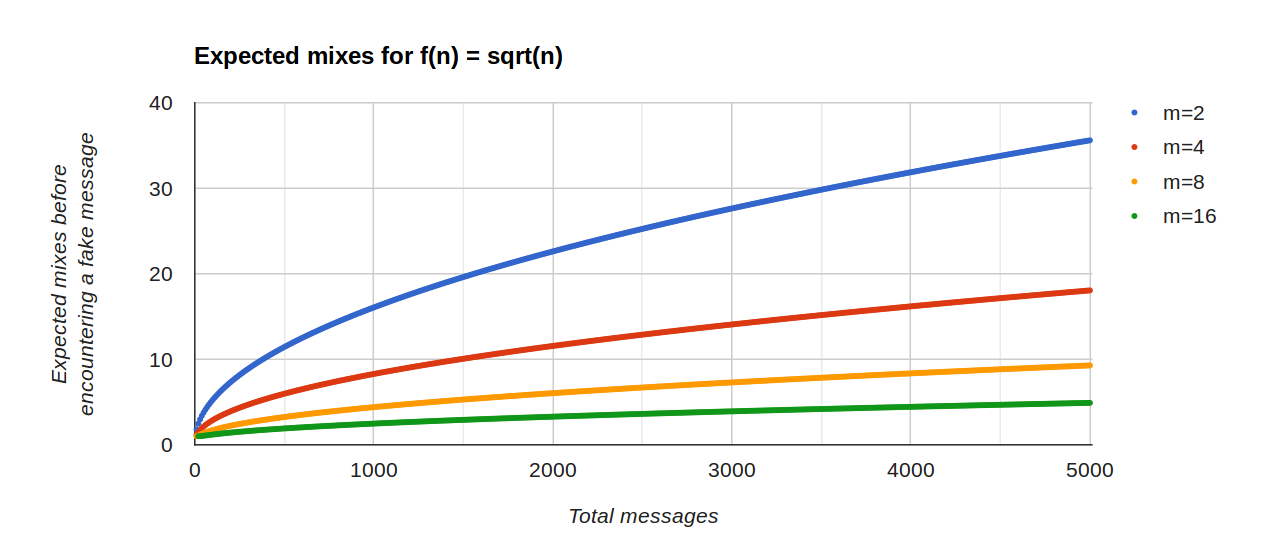
\includegraphics[width=\textwidth]{sqrtn}

With high bandwidth, including only $\sqrt(n)$ fake messages could be feasible: with a batch size of 16, even at a total mailbox size of 5000 we would still encounter a fake message about every 5 mixes.


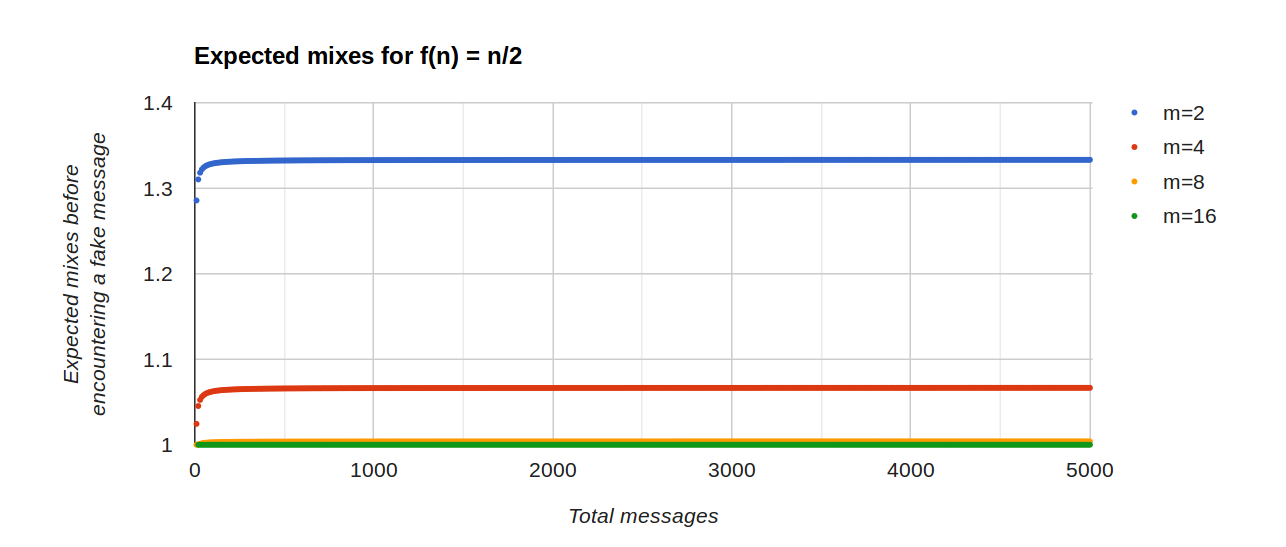
\includegraphics[width=\textwidth]{nover2}

With a linear function where half the mailbox is composed of fake messages, we achieve spectacular rates of message inclusion, of course, but we waste much space in the mailbox.

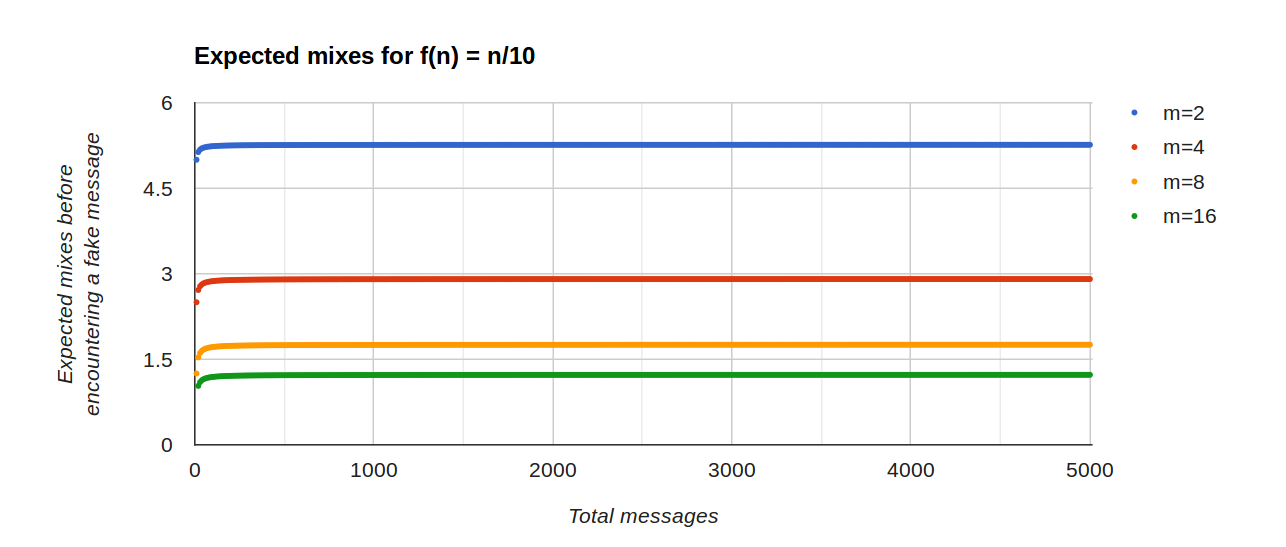
\includegraphics[width=\textwidth]{nover10}

Changing the constant on our linear function, we can save substantial mailbox space while still achieving very reasonable delays. With only one tenth of messages being decoy messages, we will encounter a fake message about every 3 mixes with a batch size of only 4, and just over every 1.5 mixes with a batch size of 8.

While we could achieve reasonable rates in this way, we assume here that a mix is effective \---- that all messages included in it are of the same size, and that fetching patterns do not reveal further information. But neither of these are the case in practice. For the latter, assume that client A performs a mix. If client B soon after that fetches a message that was output from that mix, the server knows that a message was received. For the former, breaking up messages into correlated chunks will again reveal which messages are real. Bucketing solutions where messages are padded to a variety of sizes might be possible, but since message sizes follow a long tail distribution, a bucketing strategy will likely waste a good deal of space at the longer end of the spectrum. For both of these reasons, an ORAM-like protocol is needed to ensure full metadata protection.


\subsubsection{ORAM-like protocol}

Is applying an ORAM-like protocol feasible? Recall that an ORAM-like protocol is one where patterns of data access are hidden from the server. To do this, larger messages must be broken down into chunks of a set size. With a long tail distribution, this is feasible in most cases. Chunks could easily be tracked inside the INDEX, with each piece being fetched sequentially. Using Path ORAM \cite{stefanov2013path}, for a block size of $\Omega (\log ^2 N)$ bits where $N$ is the total number of blocks, there is a bandwidth cost of $O(\log N)$ blocks, and a required $O(\log N)\omega(1)$ blocks stored on the client. Accessing $O(\log N)$ messages per required desired access is a reasonable cost, particularly relative to the overhead of mixing.

While most ORAM abstractions map trivially onto IMAP operations, a significant difference is that most ORAM techniques are constructed for a fixed-size store. A trivial way to handle this is to initially seed the mailbox to near-full capacity, and disallow emails to arrive from legacy pathways. We can do better though, using Resizable Tree-Based ORAM as described in \cite{moatazresizable}. This protocol provides alloc and free operations in addition to read/write, in a way that leaks only the current number of elements, and is thus the appropriate construction for the abstractions of an IMAP-like system.

\section{Attacks and Countermeasures}

Even with all precautions previously described put into place, there are still potential attacks that \project could be vulnerable to.

\subsection{Multiple Client Signup INDEX Rollback}

Given the current SEQUENCE NUMBER mechanism, a server can force a new client to accept a previous version of the system, and use this acceptable to roll back existing clients as well. Here we describe the steps involved in this attack.

\begin{enumerate}
\item Client A signs up and makes changes, incrementing the SEQUENCE NUMBER is 10.
\item The IMAP server rolls back the entire system to when the SEQUENCE NUMBER was 8.
\item Client B signs up and accepts that the initial sequence number is 8.
\item Client B makes changes such that the SEQUENCE NUMBER is 12.
\item Client A connects to the server, sees that the sequence number is 12 (which is greater than 10), and accepts the INDEX. Client A assumes that Client B made changes that undid the results of INDEXes 9 and 10 before applying updates 11 and 12.
\end{enumerate}

\subsubsection{Defense}
When a new client signs up, either manually inspect the contents to ensure that they are in the expected state or display the current sequence number on both an existing client and the new client for a user to compare.

\section{Discussion}
As discussed in Section~\ref{architecture}, every client of an IMAP server must upgrade to \project if any client does so. Therefore, for this technology to spread, \project must be available across platforms on initial release, as a standard modern user expects to be able to check his or her email across devices and email clients. One potentially opportune venue for this is in an enterprise setting. Many businesses require a particular software stack for their employees, often employing IT staff to manage the installation and upkeep on behalf of all workers. Additionally, a business stands to gain much from employing metadata protection. A company involved in manufacturing a product may wish to hide from which vendor it is buying its components before the product's release; disclosure of an email exchange with a particular vendor could compromise this secret. Today, these companies often run their own mail servers to manage such leakages, imposing extraneous time and technology costs on them. With \projectnospace, a company could instead either purchase or build only a mail client, lightening their IT burden.

For rollback detection and caching, the client of \project must be run on a trusted host. In this implementation, the client is a webmail service. Theoretically, a mail provider could run a webmail client that uses \projectnospace, serving Javascript to visitors that enables in-browser encryption and decryption \cite{wagner}. Send queue and other caches could be saved in encrypted form on the webmail server, and only key and rollback prevention information stored in-browser. This could encourage more widespread usage by simplifying setup and reducing downloads, making the overall system more usable.

\section{Summary}
With \projectnospace, we present a solution that efficiently upgrades the IMAP protocol to support the storage and synchronization of emails while preserving end-to-end metadata security in the presence of an adversarial server. \project can be invisibly rolled out to users, providing metadata security for an integral component of the email ecosystem.

\pagebreak

\section*{Acknowledgements}

\pagebreak

\bstctlcite{bstctl:etal, bstctl:nodash, bstctl:simpurl}
\bibliographystyle{IEEEtranS}
\bibliography{references}

\end{document}



